%%%%%%%%%%%%%%%%%%%%%%%%%%%%%%%%%%%%%%%%%%%%%%%%%%%%%%%%%%%%%%%%%%%%%%%%%%%%%%%%
% LaTeX Document for arXiv Submission
% Title: Generalized Reversible Computation: A New Paradigm for Unifying Software Construction and Evolution
%%%%%%%%%%%%%%%%%%%%%%%%%%%%%%%%%%%%%%%%%%%%%%%%%%%%%%%%%%%%%%%%%%%%%%%%%%%%%%%%

\documentclass[11pt]{article}

% PACKAGES
\usepackage[utf8]{inputenc}
\usepackage[T1]{fontenc}
\usepackage{amsmath, amssymb}
\usepackage{graphicx}
\usepackage[a4paper, margin=1in]{geometry}
\usepackage{hyperref}
\usepackage{booktabs}
\usepackage{caption}
\usepackage{listings}
\usepackage{enumitem}
\usepackage{tabularx}
\usepackage{longtable}
\usepackage{xcolor}
\usepackage{array}
\usepackage{newunicodechar}
\usepackage{url}

% CONFIGURATION
\Urlmuskip=0mu plus 1mu 

% arXiv-friendly hyperref setup
\hypersetup{
    colorlinks=false,
    pdfborder={0 0 0},
    pdftitle={Generalized Reversible Computation: A New Paradigm for Unifying Software Construction and Evolution},
    pdfauthor={Canonical}, % --- YOU CAN CHANGE THIS ---
    pdfsubject={Computer Science},
    pdfkeywords={Generalized Reversible Computation, Delta-Oriented Programming, Metaprogramming, Model-Driven Engineering, Software Product Lines, Domain-Specific Languages, Recursive Fractal-like Construction, Domain-Driven Design, Minimal Information Expression, Software Configuration Management, Variability Management, Software Product Line Engineering, Compositional Software Development}
}

% Listings setup for code blocks
\definecolor{codegreen}{rgb}{0,0.6,0}
\definecolor{codegray}{rgb}{0.5,0.5,0.5}
\definecolor{codepurple}{rgb}{0.58,0,0.82}
\definecolor{backcolour}{rgb}{0.98,0.98,0.96}

\lstdefinestyle{mystyle}{
    backgroundcolor=\color{backcolour},   
    commentstyle=\color{codegreen},
    keywordstyle=\color{magenta},
    numberstyle=\tiny\color{codegray},
    stringstyle=\color{codepurple},
    basicstyle=\ttfamily\footnotesize,
    breakatwhitespace=false,         
    breaklines=true,                 
    captionpos=b,                    
    keepspaces=true,                 
    numbers=left,                    
    numbersep=5pt,                  
    showspaces=false,                
    showstringspaces=false,
    showtabs=false,                  
    tabsize=2,
    frame=single,
    framerule=0pt,
    framesep=5pt,
    framexleftmargin=5pt,
    literate={_}{\textunderscore}1
}
\lstset{style=mystyle}

% Define languages for listings
\lstdefinelanguage{YAML}{
  basicstyle=\ttfamily\footnotesize,
  comment=[l]{\#},
  commentstyle=\color{gray},
  morestring=[b]',
  morestring=[b]",
  stringstyle=\color{red},
  showstringspaces=false
}

\newcommand\ProcessThreeDashes{\llap{\color{blue}\bfseries---}}

\renewcommand{\topfraction}{0.9}
\renewcommand{\bottomfraction}{0.9}
\renewcommand{\textfraction}{0.05}
\renewcommand{\floatpagefraction}{0.8}

\lstdefinelanguage{PythonPseudocode}{
    keywords={function, return, if, else, for, in, and, or, not, del, is, NULL, clone, getAttributes, setAttribute, getChildren, setChildren},
    keywordstyle=\color{blue}\bfseries,
    comment=[l]{\#},
    commentstyle=\color{codegreen},
    stringstyle=\color{red},
    sensitive=true,
    morestring=[b]',
    morestring=[b]",
    basicstyle=\ttfamily\footnotesize,
}

% Custom column type for tables
\newcolumntype{L}[1]{>{\raggedright\let\newline\\\arraybackslash\hspace{0pt}}p{#1}}

% DOCUMENT START
\begin{document}

\title{\textbf{Generalized Reversible Computation: A New Paradigm for Unifying Software Construction and Evolution}}
\author{Canonical \\ \texttt{canonical\_entropy@163.com}}
\date{\today}

\maketitle

\begin{abstract}
This paper proposes and systematically elucidates the theory of Generalized Reversible Computation (GRC), a new paradigm for unifying software construction and evolution. Unlike traditional logical reversible computation, which focuses on runtime execution, GRC extends the principle of "reversibility" from runtime to the construction process across the entire software lifecycle. Its core principle is the elevation of the \textbf{Structured Delta} to a first-class citizen, systematically taming the complexity of software evolution through a unified construction formula: $\text{App} = \text{Generator}\langle\text{DSL}\rangle \oplus \Delta$. This paper first defines the theoretical scope of GRC from first principles, positioning it as a computational framework for managing complexity by drawing an analogy to the Dirac (Interaction) Picture in physics. Building on this foundation, we detail GRC's core mechanisms, including its recursive fractal-like construction properties and delta composition based on algebraic operations. We demonstrate the explanatory power of GRC theory by reinterpreting Domain-Driven Design (DDD) and providing a unified analysis of modern engineering practices such as Docker, Kustomize, and OpenUSD. Finally, we validate the engineering feasibility and potential advantages of GRC through a canonical implementation in the Nop Platform and a case study of retrofitting a large-scale banking core system. We contend that GRC offers a systematic, scalable, and theoretically-grounded solution to the two fundamental challenges in software engineering: "complexity" and "evolution." By articulating this framework and providing initial validation, this paper aims to lay the groundwork for its further formalization and widespread application.
\end{abstract}

\vspace{1em}
\noindent\textbf{Keywords}: Generalized Reversible Computation, Delta-Oriented Programming, Metaprogramming, Model-Driven Engineering, Software Product Lines, Domain-Specific Languages, Recursive Fractal-like Construction, Domain-Driven Design, Minimal Information Expression, Software Configuration Management, Variability Management, Software Product Line Engineering, Compositional Software Development

\section{Introduction: From Computability to the Challenge of Complexity}

In the history of computer science, the Turing Machine and Lambda Calculus laid the theoretical foundation for "computability," answering the fundamental question of "what is computable?" However, as software systems have evolved from isolated algorithms into intricate ecosystems, our core challenge has shifted from "computability" to "complexity management."

Several long-standing challenges in software engineering can be distilled into three fundamental dichotomies:
\begin{itemize}
    \item The conflict between \textbf{standardization and customization}: How to satisfy individual needs while maintaining the stability of a core product.
    \item The conflict between \textbf{reuse and evolution}: How to support the continuous evolution of a system while reusing existing assets.
    \item The conflict between \textbf{entropy and control}: How to systematically govern software decay and control the growth of complexity.
\end{itemize}

To address these, this paper formally introduces \textbf{Generalized Reversible Computation (GRC)}. The core idea of GRC is that the construction and evolution of any complex software system can be described by a single, unified construction formula. It asserts that a system can always be decomposed into a predictable "ideal backbone" built from a standardized \textbf{model} via a deterministic \textbf{generator}, and the superposition of one or more structured \textbf{deltas} that encapsulate all non-ideal, customized, and evolutionary modifications. This core idea can be formally expressed as:
\[
\text{App} = \text{Generator}\langle\text{DSL}\rangle \oplus \Delta
\]

Before delving into the theoretical system, we provide a brief glossary of the core concepts discussed in this paper to help readers build a clear cognitive map.

\begin{longtable}{@{} >{\bfseries}L{4.5cm} >{\raggedright}L{3.5cm} p{0.5\textwidth} @{}}
\caption{Glossary of Core Concepts} \label{tab:glossary} \\
\toprule
\textbf{Term} & \textbf{English/Symbol} & \textbf{Definition \& Explanation} \\
\midrule
\endfirsthead
\multicolumn{3}{c}%
{{\bfseries \tablename\ \thetable{} -- continued from previous page}} \\
\toprule
\textbf{Term} & \textbf{English/Symbol} & \textbf{Definition \& Explanation} \\
\midrule
\endhead
\bottomrule
\endfoot
Generalized Reversible Computation & Generalized Reversible Computation (GRC) & The new paradigm proposed in this paper. It extends the principle of "reversibility" from runtime to the \textbf{entire process of software construction and evolution}, with a core focus on systematically managing complexity through algebraic delta operations. \\
\addlinespace
Core Construction Formula & $\text{App} = \text{Generator}\langle\text{DSL}\rangle \oplus \Delta$ & The mathematical cornerstone of GRC. It asserts that any software application (App) can be decomposed into a \textbf{predictable foundation built from a Generator and a DSL}, combined with one or more \textbf{Structured Deltas ($\Delta$) that encapsulate all changes}. \\
\addlinespace
Structured Delta & Structured Delta ($\Delta$) & A \textbf{first-class citizen} in GRC. It is a \textbf{structured data packet} that encapsulates evolutionary operations--additions, deletions, modifications--on a base model. Unlike a text `diff`, it operates at the \textbf{semantic level} and possesses algebraic properties. \\
\addlinespace
Generator & Generator & The deterministic transformation function in the GRC formula. It is responsible for reading a \textbf{Domain-Specific Language (DSL)} and "compiling" or "interpreting" it into a predictable, standardized "ideal backbone" of the system. \\
\addlinespace
Domain-Specific Language & Domain-Specific Language (DSL) & The carrier of the "\textbf{semantic coordinate system}" in GRC. It provides a stable, business-meaningful structure for software artifacts, enabling deltas ($\Delta$) to have \textbf{precise and robust addressing anchors}. \\
\addlinespace
Reversible Merge Operator & Reversible Merge Operator ($\oplus$) & The core algebraic operation used to apply a delta ($\Delta$) to a base model. It is designed to be \textbf{non-invasive} and theoretically supports an \textbf{inverse operation} ($\text{Base} = \text{App} - \Delta$), enabling the precise calculation and stripping of changes. \\
\end{longtable}

At a high level, this core construction principle can be understood as a new architectural paradigm. \textbf{As illustrated in Figure \ref{fig:delta_arch}}, a typical layered software system, regardless of its internal divisions (e.g., infrastructure, core engine, and business application layers), can be enhanced by a new, orthogonal "delta customization" dimension. This Delta dimension is the manifestation of the structured delta $\Delta$ in the GRC formula. It acts like a unified control bus, capable of non-invasively modifying, replacing, or extending any layer of the system, thereby converging scattered, ad-hoc customization requirements into a systematic, manageable framework.

\begin{figure}[htbp]
    \centering
    % NOTE: You must convert the SVG file to PDF or PNG and place it in the 'ddd' subdirectory.
    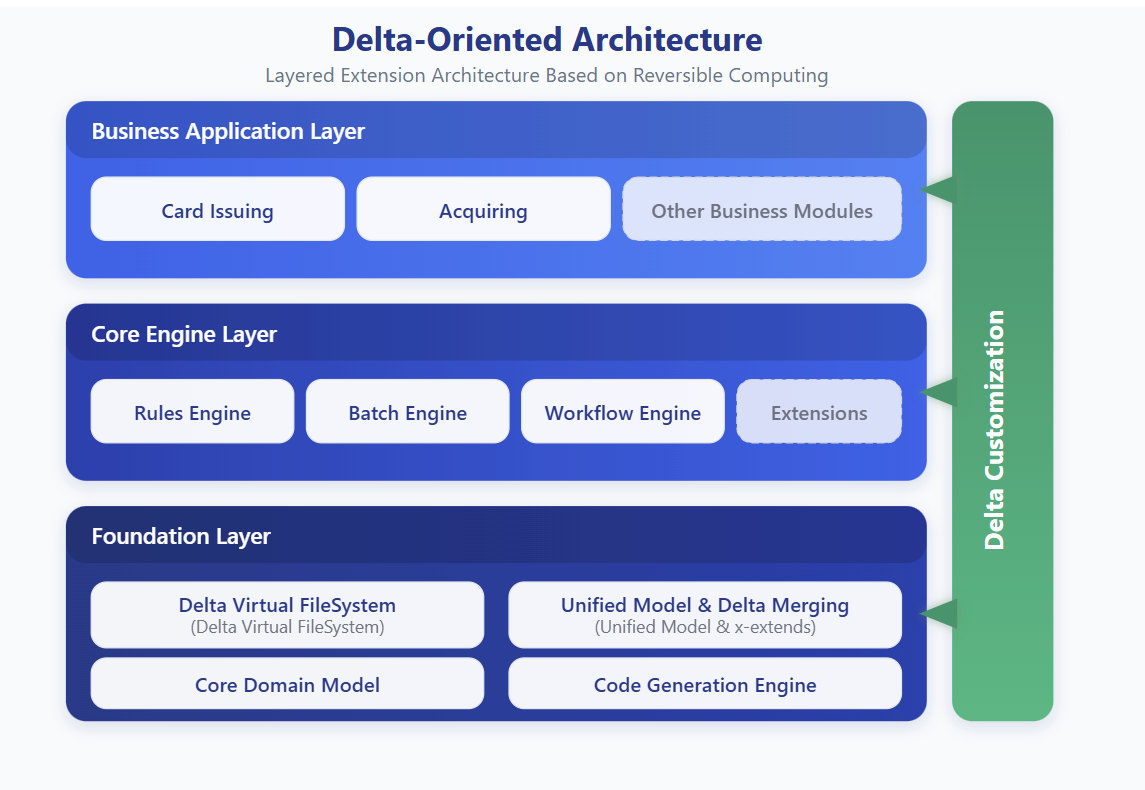
\includegraphics[width=0.8\textwidth]{ddd/delta-oriented-arch.png}
    \caption{A Top-Level Architectural Metaphor for GRC--A Layered Architecture with Delta Customization. This diagram illustrates the core idea of the GRC paradigm: a traditional, vertically layered software system (Infrastructure, Core Engine, Business Application) is non-invasively enhanced by an orthogonal "Delta Customization" dimension that cuts across all layers. This Delta dimension corresponds to the $\Delta$ in the GRC formula, providing a unified and scalable mechanism for system evolution and variability management.}
    \label{fig:delta_arch}
\end{figure}

The main contributions of this paper are:
\begin{enumerate}
    \item \textbf{Paradigm Establishment and Positioning}: We systematically define GRC for the first time, establish its conceptual foundation as a computational framework through analogies with methodologies in physics, and clarify its relationship with related work such as DOP and MDA.
    \item \textbf{Elucidation of the Theoretical Core}: We detail GRC's recursive fractal-like construction properties, its three dimensions of reversibility, and the foundation of its delta algebra.
    \item \textbf{Demonstration of Unifying Explanatory Power}: Starting from GRC's first principles, we reinterpret Domain-Driven Design (DDD) and reveal the unified construction laws underlying modern practices like Docker and OpenUSD.
    \item \textbf{Engineering Practice Validation}: We demonstrate the engineering feasibility, potential advantages, and universality of GRC theory through its canonical implementation in the Nop Platform and a case study of a large-scale enterprise system.
\end{enumerate}

We begin by systematically articulating the substance of GRC, starting with its theoretical positioning and related work.

\section{Theoretical Positioning and Related Work}

\subsection{Conceptual Demarcation of Generalized Reversible Computation}
To precisely define the theoretical scope of Generalized Reversible Computation (GRC), it is essential to distinguish it clearly from other "reversibility" concepts in computer science:

\begin{itemize}
    \item \textbf{Physical Reversible Computing}: This field focuses on how to build extremely low-energy computing hardware using reversible processes at the level of physical laws. Its theoretical basis can be traced to Landauer's principle, which clarifies the necessary link between information erasure and energy dissipation \cite{landauer1961}.
    \item \textbf{Logical Reversible Computation (LRC)}: A branch of theoretical computer science concerned with whether computational steps at runtime have a strict logical bijection, meaning each computational state has a unique successor and predecessor. Bennett proved that any computational process can, in principle, be transformed into a logically reversible form \cite{bennett1973}.
    \item \textbf{Generalized Reversible Computation (GRC)}: The software construction paradigm proposed in this paper. It extends the principle of "reversibility" from the execution logic at \textbf{runtime} to the \textbf{design/build-time} activities across the entire software lifecycle. The core issue for GRC is not to eliminate all irreversibility, but rather, in a software engineering world that is macroscopically entropic, how to use reversible, algebraic construction operations as a core mechanism to systematically organize and tame unavoidable irreversibility.
\end{itemize}

Therefore, GRC and LRC are not in competition but are concepts that focus on different levels. LRC can be seen as a theoretical special case of GRC where the construction dimension is greatly simplified to focus solely on runtime execution steps. GRC is concerned with the broader construction dynamics that encompass the entire process of software design, implementation, deployment, and evolution.

\subsection{Systematic Comparison with Related Work}

The core idea of Generalized Reversible Computation (GRC) was independently conceived in 2007, inspired not by mainstream software engineering paradigms but by methodologies from theoretical physics for handling complex many-body systems (see Section 4.1). In the process of systematizing its theory for this paper, we reviewed the academic literature in software engineering and discovered that many similar explorations have been independently undertaken in fields such as Model-Driven Engineering (MDE), Software Product Lines (SPL), and Feature-Oriented Programming (FOP).

This phenomenon of "convergent evolution"--different paths leading to similar solutions--suggests to some extent that "delta-oriented" and "generative" construction may be an effective pattern for tackling software complexity. The purpose of this section is not only to clarify the origins of GRC's ideas but also to place it within a broader academic coordinate system. By comparing it with these prior works, we aim to reveal GRC's distinct characteristics in terms of theoretical completeness, algebraic rigor, and unifying power. We argue that many existing construction theories can be understood as incomplete implementations of the core GRC formula $\text{App} = \text{Generator}\langle\text{DSL}\rangle \oplus \Delta$ along different dimensions.

\subsubsection{Model-Driven Engineering (MDE): Generation without Deltas}

Model-Driven Engineering (MDE), and its early concrete implementation, Model-Driven Architecture (MDA) \cite{omg2003}, represented a major paradigm exploration in software engineering to raise the level of abstraction from code to models \cite{schmidt2006}. Its core pattern can be abstracted as $\text{App} = \text{Transformer}(\text{Model})$, which is highly consistent in spirit with the $\text{Generator}\langle\text{DSL}\rangle$ part of the GRC formula, as both recognize "generation" as a core means of systematic construction.

MDE significantly improves productivity and consistency by making the model the Single Source of Truth and automatically generating code and other artifacts from it. However, a well-recognized challenge in classic MDE methods is their relative rigidity in handling "exceptions" or "customization" requirements that deviate from the core model. GRC aims to systematically solve this problem by introducing a structured delta mechanism ($\Delta$) that collaborates orthogonally with the generation process. It allows for non-invasive, traceable evolutionary modifications without corrupting the core model (the output of $\text{Generator}\langle\text{DSL}\rangle$), thus completing a crucial missing piece in MDE.

\subsubsection{Delta-Oriented/Feature-Oriented Programming (DOP/FOP): Deltas without a Complete Coordinate System}

Feature-Oriented Programming (FOP) \cite{batory2004} and its subsequent evolution, Delta-Oriented Programming (DOP) \cite{schaefer2010}, are primarily used to manage variability in Software Product Lines (SPL) \cite{pohl2005}. These paradigms grasp one half of the truth in the GRC formula--the $\Delta$--by reifying "change" itself into manipulable "feature" or "delta" modules.

Their classic pattern, $\text{Product} = \text{Core} \oplus \text{Deltas}$, reveals their theoretical limitations:
\begin{enumerate}
    \item \textbf{The Unspecified Core}: The origin and construction method of the `Core` are not theorized; it is usually assumed to be a pre-existing, manually crafted artifact.
    \item \textbf{Lack of a Stable Semantic Coordinate System}: The delta operations in DOP/FOP typically act on unstable code structures defined by General-Purpose Languages (GPLs), and their addressing mechanisms (e.g., matching based on code patterns) are relatively fragile. Although some research has explored the use of DSLs in FOP \cite{kaestner2009}, the role of the DSL is more auxiliary.
\end{enumerate}

GRC systematically addresses these two problems with its other two theoretical pillars: the `Generator` and the `DSL`. $\text{Generator}\langle\text{DSL}\rangle$ provides a deterministic theoretical origin for the `Core`, while the DSL itself, through its inherent structure and domain semantics, constructs a stable "\textbf{semantic coordinate system}" that provides robust anchors for delta operations.

\subsubsection{Aspect-Oriented Programming (AOP): Spatial Commonality vs. Temporal Similarity}

Aspect-Oriented Programming (AOP) \cite{kiczales1997} introduced a mechanism for modularizing cross-cutting concerns. From a GRC perspective, AOP can be seen as a form of unstructured delta injection.

AOP and GRC differ in the dimension of "change" they capture. AOP's Pointcuts primarily capture "\textbf{spatial commonality}"--concerns that cut across different modules at the same point in time. In contrast, GRC's deltas ($\Delta$) primarily capture the "\textbf{temporal similarity}" of the same artifact during its evolution. An AOP pointcut is a query semantic, and its scope of effect may change due to code refactoring. A GRC delta, however, is a construction semantic; its target is deterministic, based on precise domain coordinates defined by a DSL.

\subsubsection{Version Control Systems (VCS): Textual Deltas with Weaker Algebraic Properties}

Modern Version Control Systems (VCS) like Git represent the most successful application of delta-oriented thinking in engineering practice. Their `diff/patch` mechanism has profoundly influenced a generation of developers, and academia has extensively mined and analyzed VCS history data \cite{gousios2013}.

However, GRC seeks to achieve a paradigm upgrade over VCS by elevating the delta from the \textbf{"syntactic/text space" to the "semantic/model space"} and endowing it with robust algebraic properties. Git's `diff` and GRC's $\Delta$ differ in their mathematical properties:
\begin{itemize}
    \item \textbf{Different Delta Spaces}: Git's deltas are defined in the \textbf{line-based text space} and lack business semantics. GRC's deltas are defined in the \textbf{domain model space}, where the minimal unit of operation is a semantic node with clear business meaning.
    \item \textbf{Lack of Closure}: A Git `merge` can result in a "Conflict," producing an abnormal structure that falls outside the space of "valid source code." This requires manual intervention and breaks the closure of the operation. GRC's merge operator $\oplus$ is designed to be closed within the model space.
    \item \textbf{Lack of Associativity}: A Git delta (patch) is tightly coupled to a specific baseline version and cannot be independently composed in a way like $(\text{patch}_1 \oplus \text{patch}_2) \oplus \text{patch}_3 = \text{patch}_1 \oplus (\text{patch}_2 \oplus \text{patch}_3)$. This prevents it from having general-purpose composability.
\end{itemize}

In summary, Git provides valuable but mathematically weak management of text-level deltas. GRC, by elevating deltas to \textbf{semantic-level entities} with well-behaved algebraic properties, makes large-scale, automated, and predictable software construction and evolution possible.

\subsubsection{Language Workbenches: Unified Metamodel vs. Language Composition}

JetBrains MPS (Meta Programming System), as a paradigm of a Language Workbench \cite{erdweg2013, fowler2005lw}, has at its core the idea of decoupling developers from the underlying text syntax through a \textbf{Projectional Editor}, allowing them to directly manipulate the Abstract Syntax Tree (AST). It builds a dedicated, highly customized development experience for each DSL and then aggregates these independent capabilities through \textbf{Language Composition}. This entire methodology is also known as Language-Oriented Programming (LOP) \cite{dmitriev2004}.

While GRC also makes extensive use of DSLs, its theoretical starting point and construction philosophy are fundamentally different. GRC posits that since any language can ultimately be parsed into an AST, normalizing these heterogeneous ASTs into a \textbf{unified metamodel} (in the Nop Platform, this is the XNode, an engineered implementation of the universal structure of Lisp S-expressions) is a natural and powerful abstraction. Based on this, GRC provides a more lightweight and algebraically complete path to achieving the capabilities of a language workbench.

The paradigmatic differences between GRC and MPS can be analyzed through several key points:

\begin{enumerate}
    \item \textbf{Unified Metamodel \& Homomorphic Metaprogramming}: MPS maintains separate AST structures for each language. In contrast, GRC proposes a unified XNode metamodel, making \textbf{transformations on the model (metaprogramming) homomorphic to the structure of the model itself}. This allows the `Generator` to be implemented as a mechanism akin to Lisp macros, performing Turing-complete transformations at the unified AST level, with capabilities far exceeding simple code generation.
    \item \textbf{Multiple, Reversible Representations}: In GRC, \textbf{the same information can have multiple different representations}. The text of a DSL is its \textbf{textual representation}, while a complex interactive interface is its \textbf{visual representation}. These representations can, in theory, be freely and reversibly converted between one another. In MPS, the projectional editor is part of the "language definition," whereas in GRC, representations are separate from the model. A powerful example is that the GRC framework can automatically provide an Excel representation for *all* DSLs. The necessary parsing and validation logic can be supplemented through a mapping definition. \textbf{Crucially, this mapping is flexible; it matches data purely based on attribute names without specifying fixed cell locations.} Thus, the system can not only generate but also reliably reverse-parse structured Excel files, allowing users to directly edit complex DSL tree structures using Excel. This ability to provide robust, universal editing methods for any DSL at low cost is a significant advantage of the GRC paradigm.
    \item \textbf{Generator as Representation Constructor}: Based on the above, the core GRC formula $\text{App} = \text{Generator}\langle\text{DSL}\rangle \oplus \Delta$ gains a deeper interpretation. The \textbf{`Generator`} here is no longer just a code generator; it is generalized to be \textbf{any transformer from the unified metamodel to a specific representation}. This includes the process of constructing a "projectional editor." At the implementation level, this can be achieved with great generality and flexibility: as a rendering engine traverses an XNode tree, \textbf{it can dynamically look up and load the corresponding UI control from a specified control library (`control.xlib`) based on each node's tag name (`tagName`)}. For example, a `<wf:send-task>` node could be mapped to a graphical block displaying "Send Task." By providing different control libraries--one for web rendering, another for a desktop IDE plugin--one can \textbf{generate completely different-looking and -behaving visual editors for the same XNode model data}.
    \item \textbf{Explicit Delta Algebra}: This is GRC's most unique theoretical contribution. MPS itself does not have a built-in concept of "delta merging and decomposition." GRC, by defining the $\oplus$ merge operator and the structured delta $\Delta$ on top of the unified XNode metamodel, provides an explicit, algebraically well-behaved language of operations for model evolution, customization, and composition.
\end{enumerate}

The table below summarizes the differences in the core mechanisms of the two paradigms:

\begin{table}[htbp]
\centering
\caption{Comparison of GRC and JetBrains MPS Paradigms}
\begin{tabularx}{\textwidth}{@{} l X X @{}}
\toprule
\textbf{Dimension} & \textbf{JetBrains MPS} & \textbf{Generalized Reversible Computation (GRC)} \\
\midrule
\textbf{Theoretical Focus} & Projectional Editing, Language Composition & \textbf{Unified Metamodel, Multiple Representations, Delta Algebra} \\
\addlinespace
\textbf{Core Structure} & Separate, typed ASTs for each language & Unified XNode metamodel (embodying Lisp S-expression ideas) \\
\addlinespace
\textbf{Representation Mechanism} & Language and editor are tightly coupled & \textbf{Same XNode reversibly mapped to multiple representations via control libraries} \\
\addlinespace
\textbf{Meaning of Generator} & Primarily a code generator & \textbf{Representation Constructor (incl. visual editors) \& Homomorphic Macros} \\
\addlinespace
\textbf{Evolution Mechanism} & Relies on language module's own version management & \textbf{Explicit, computable evolution based on delta algebra} \\
\addlinespace
\textbf{Paradigm Positioning} & Heavyweight, complete language workbench & \textbf{A lightweight, algebra- and metaprogramming-based framework for realizing a language ecosystem} \\
\bottomrule
\end{tabularx}
\end{table}

In conclusion, GRC does not simply replicate or replace language workbenches. By returning to the universal structural idea of Lisp S-expressions and creatively supplementing it with the concepts of "delta algebra" and "multiple reversible representations," it provides a more fundamental and unified theoretical framework for both the construction (via `Generator` creating representations) and evolution (via `$\oplus \Delta$` applying changes) of software.

\subsubsection{Conclusion: A More Fundamental Construction Paradigm}

GRC is not a simple combination of the aforementioned theories but offers a more fundamental and general construction paradigm. By introducing the three cornerstones of a \textbf{Generator}, an \textbf{Algebraic Delta}, and a \textbf{Semantic Coordinate System (via DSL)}, it unifies other theories as special cases or approximations under different constraints. From this perspective, the history of software construction paradigms can be interpreted as a gradual process of exploration and convergence toward the complete form of $\text{App} = \text{Generator}\langle\text{DSL}\rangle \oplus \Delta$.

\section{The Core Mechanisms of GRC: Recursive Fractals and Delta Algebra}

The core mechanisms of GRC theory are built upon three closely related cornerstones: first, the foundational paradigm of "generation and delta" synergy; second, the algebraic principle that unifies "construction" and "evolution"; and third, the recursive fractal-like construction law that reveals software's self-similarity. Together, these form the operational framework for taming complexity.

\subsection{The Core Paradigm: A Binary Synergy of Generation and Delta}

The GRC construction paradigm, embodied by the unified formula $\text{App} = \text{Generator}\langle\text{DSL}\rangle \oplus \Delta$, is essentially an idea of decomposition into a "\textbf{base + perturbation}." An abstract analogy for this idea is the elevation of the software construction paradigm from OOP's `Map = Map extends Map` to GRC's `Tree = Tree x-extends Tree`. This represents an expansion of the operational space from a flat class structure to a hierarchical system model tree, and an upgrade of the operator from simple property overriding to an algebraically complete, reversible merge.

This translates into a concrete technical implementation path:

\begin{verbatim}
App = Delta x-extends Generator<DSL>
\end{verbatim}

Where:
\begin{itemize}
    \item \textbf{Generator<DSL>}: The idealized backbone of the system, providing a standard, default structure.
    \item \textbf{Delta}: A structured delta defining all customizations and specializations to the standard base.
    \item \textbf{x-extends}: The reversible merge operator, an algebraic upgrade to traditional inheritance mechanisms.
\end{itemize}

\subsection{Construction is Evolution: The Unifying Principle of $A = \emptyset \oplus A$}

The algebraic identity $A = \emptyset \oplus A$, in the context of GRC, reveals the \textbf{intrinsic unity of software construction and evolution}.

In traditional software engineering, "project initialization" (construction) and "feature changes" (evolution) are typically treated as two distinct activities, using different mental models and toolsets. GRC, by elevating the "delta" to a first-class citizen, perfectly unifies them under the same algebraic law.

Let's translate $A = \emptyset \oplus A$ into the language of GRC:
\begin{itemize}
    \item \textbf{A (left side)}: Represents a final, runnable \textbf{Application}.
    \item \textbf{$\emptyset$ (empty set symbol)}: Represents a \textbf{"Zero Model"} or \textbf{"Empty Baseline."} It is the \textbf{Identity Element} in the GRC delta algebra system, a logically existing structure containing zero information.
    \item \textbf{$\oplus A$ (right side)}: Here, $A$ is no longer the final application entity but the \textbf{"Genesis Delta."} It is a massive, complete delta $\Delta_A$ that contains \textbf{all the information} needed to create the entire application $A$ from "nothing."
\end{itemize}

Thus, the profound meaning of $A = \emptyset \oplus A$ in the GRC context is:
\textbf{The construction process of a new application is essentially equivalent to applying a "Genesis Delta," which contains the application's entire definition, to a "Zero Model."}

Now, let's consider the system's evolution, for example, from version $V_1$ to $V_2$, which can be expressed as: $V_2 = V_1 \oplus \Delta$. Placing the two formulas side by side:

\begin{enumerate}
    \item \textbf{Construction}: $\text{App}_{V_1} = \emptyset \oplus \Delta_{\text{Genesis}}$
    \item \textbf{Evolution}: $\text{App}_{V_2} = \text{App}_{V_1} \oplus \Delta_{\text{Incremental}}$
\end{enumerate}

The unity becomes apparent: \textbf{Construction is evolution}. The construction process can be seen as \textbf{one grand evolution from a "zero baseline."} Conversely, the evolution process can be seen as \textbf{a local construction on a "non-zero baseline."}

This unifying principle brings immense engineering value:
\begin{itemize}
    \item \textbf{Conceptual Simplification}: The entire software lifecycle is simplified to a single core operation: \textbf{Apply Delta}.
    \item \textbf{Toolchain Unification}: Since the underlying law is unified, the toolchains for "construction" and "evolution" can also be unified. A single merge engine can be used both to generate an application from scratch and to apply a tiny patch to it.
    \item \textbf{Everything is a "Patch"}: A new feature, a customer customization, an emergency fix, or even the entire initial application itself, are all abstracted into independently manageable, composable, and reusable delta assets.
\end{itemize}

\subsection{Recursive Fractal-like Construction: The Principle of Self-Similarity in Software Construction}

A core insight of GRC theory is the recursive self-similarity exhibited by the software construction process: its fundamental construction formula, $Y = F(X) \oplus \Delta$, acts as an invariant pattern that permeates all levels, from macroscopic system architecture to microscopic function implementation. We use the metaphor of a \textbf{fractal-like} structure to describe this self-repeating pattern, referring to constructional self-similarity rather than a strict mathematical geometric concept.

This recursiveness is evident across four key dimensions of software construction:

\subsubsection{Vertical Recursion: The Multi-Stage Software Production Line}

In the vertical dimension, GRC builds a \textbf{multi-stage software production line}, breaking down complex model transformations into a series of manageable steps:

\begin{align*}
\text{XMeta} &= \Delta_{\text{meta}} \oplus \text{Generator}\langle\text{XORM}\rangle \\
\text{XView} &= \Delta_{\text{view}} \oplus \text{Generator}\langle\text{XMeta}\rangle \\
\text{XPage} &= \Delta_{\text{page}} \oplus \text{Generator}\langle\text{XView}\rangle
\end{align*}

This recursive decomposition solves a core dilemma of traditional Model-Driven Architecture (MDA): it allows one to avoid striving for perfect coverage of all details during modeling. Instead, one can build a core generator that handles 80\% of common scenarios, while the remaining 20\% of special requirements are precisely injected via $\Delta$ deltas at any stage.

\textbf{Figure \ref{fig:delta_prod_line} provides a concrete example of such a multi-stage software production line.} In this example, the construction process begins with a non-technical `Excel` file, which is first converted by a generator into a structured `XORM` data model. This `XORM` model then serves as input for the next stage, used to generate a higher-level `XMeta` business model. The process continues, with `XMeta` and a business logic model (`BizModel`) combining to generate a `GraphQL` service, while also being used to generate front-end `XView` and `XPage` models, until the final user interface is rendered. The entire flow clearly demonstrates how the $Y = F(X) \oplus \Delta$ construction pattern repeats self-similarly at different levels.

\begin{figure}[htbp]
    \centering
    % NOTE: You must convert the SVG file to PDF or PNG and place it in the 'ddd' subdirectory.
    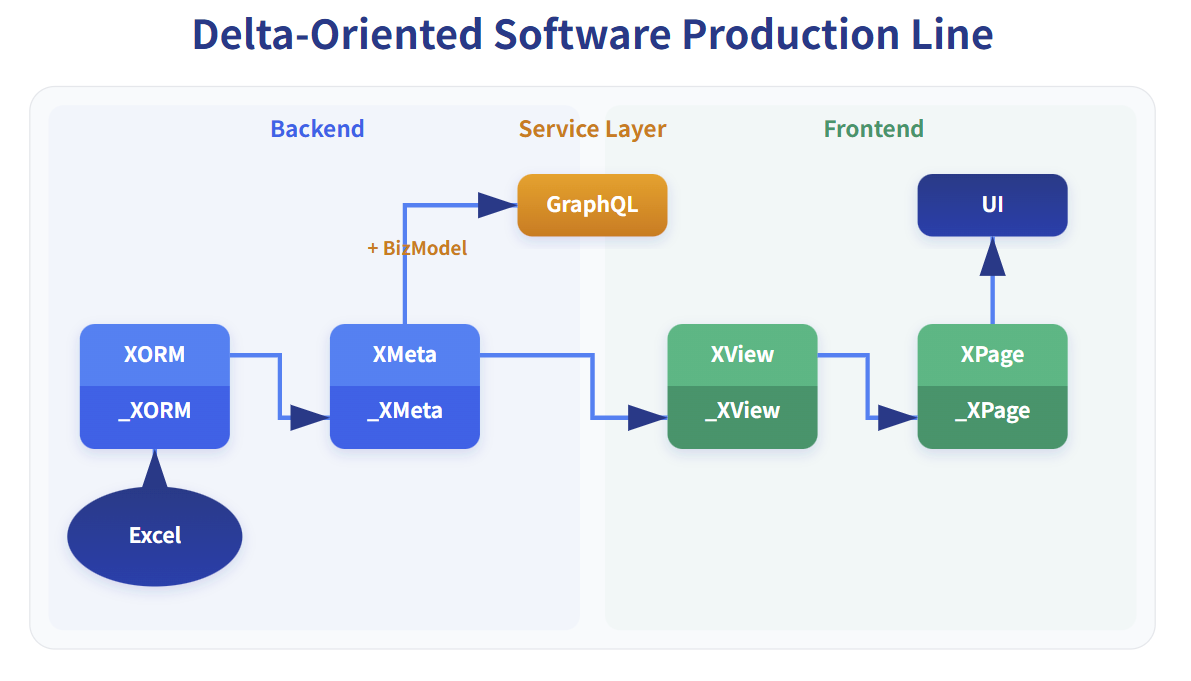
\includegraphics[width=\textwidth]{ddd/delta-pipe-line.png}
    \caption{Example of GRC's Vertical Recursive Construction--A Software Production Line from Data Source to Front-end UI. This flowchart shows the recursive application of the GRC construction formula. It starts with an Excel data source that is easy for business personnel to maintain and, through a series of deterministic generators, progressively transforms the model from one representation (`XORM`) to another (`XMeta`, `XView`, `XPage`), ultimately generating a GraphQL service and a front-end interface. At each transformation stage, customizations can be introduced by superimposing deltas (`\_XORM`, `\_XMeta`, etc.).}
    \label{fig:delta_prod_line}
\end{figure}

\subsubsection{Horizontal Recursion: The DSL Feature Vector Space}
In the horizontal dimension, GRC envisions a \textbf{DSL feature vector space}. A cross-domain business requirement can be decomposed into a set of isomorphic deltas acting on different DSL models:
\[
\text{App} = [\text{DSL}_1, \text{DSL}_2, \dots, \text{DSL}_n, \Delta_{\text{residual}}]
\]
Here, $\Delta_{\text{residual}}$ ensures the completeness of the decomposition, representing the residuals that cannot be perfectly captured by the existing DSL system.

\subsubsection{Temporal Recursion: Self-Similarity of Version Evolution}
In the time dimension, any entity in the system can be seen as a superposition of its earlier version and an evolutionary delta:
\begin{align*}
\text{Product}_{V_3} &= \Delta_{v_3} \oplus \text{Product}_{V_2} \\
\text{Product}_{V_2} &= \Delta_{v_2} \oplus \text{Product}_{V_1}
\end{align*}
This makes "change" itself a manageable, versionable, and evolvable core asset.

\subsubsection{Meta-Recursion: Bootstrapping the Construction System}
The construction system itself (`Generator`, `DSL` definitions, merge rules) also evolves according to the same invariant:
\begin{align*}
\text{MyDSL}_{v_2} &= \Delta_{\text{meta}} \oplus \text{MyDSL}_{v_1} \\
\text{Compiler}_{\text{Pro}} &= \Delta_{\text{feature}} \oplus \text{Compiler}_{\text{Base}} \\
\text{MergeRule}_{\text{New}} &= \Delta_{\text{rule}} \oplus \text{MergeRule}_{\text{Old}}
\end{align*}
The entire software world--from the final product to intermediate models, and even the construction system itself--becomes a vast, self-similar space of delta structures connected by the $\oplus$ operator.

\subsection{Delta Algebra: The Foundation for Taming Change}
The mathematical cornerstone of GRC is \textbf{Delta Algebra}. It requires the construction process to be a solvable algebraic equation, not a series of irreversible instructions. By introducing an \textbf{inverse element ($- \Delta$)} for the merge operation $\oplus$, we can achieve:
\begin{itemize}
    \item \textbf{Precise Delta Calculation}: $\Delta = \text{App} - \text{Base}$ (semantic diff).
    \item \textbf{Safe Stripping of Changes}: $\text{Base} = \text{App} - \Delta$ (semantic rebase).
\end{itemize}
This extends software reuse from the component pattern of "reusing what is identical" to the transformation pattern of "\textbf{reusing what is related}," fundamentally resolving the core conflict between a "core product and customer customizations."

\section{Theoretical Cornerstone: Analogy with Physics Methodology}

The theory of GRC is founded on an \textbf{ideological analogy} with fundamental analytical methodologies in physics.

\subsection{Analogy with the Dirac (Interaction) Picture}

GRC's "base + perturbation" decomposition idea is methodologically identical to the Dirac Picture used in quantum mechanics to handle complex interaction problems. The product of $\text{Generator}\langle\text{DSL}\rangle$ corresponds to the "exactly solvable free part" ($H_0$), while the `Delta` corresponds to the "interaction part treated as a perturbation" ($V$). This reveals that GRC is a general-purpose computational framework for tackling the problem of "complexity" in software.

\begin{table}[htbp]
\centering
\caption{Methodological Comparison of Computational Paradigms and Physics Pictures}
\begin{tabularx}{\textwidth}{@{} l X X X @{}}
\toprule
\textbf{Dimension} & \textbf{Turing Machine} & \textbf{Lambda Calculus} & \textbf{GRC Paradigm} \\
\midrule
\textbf{Analogy} & Schrödinger Picture & Heisenberg Picture & \textbf{Dirac (Interaction) Picture} \\
\addlinespace
\textbf{Philosophy} & Operators are invariant; state evolves. & State is invariant; operators evolve. & \textbf{System is decomposed into an "exactly solvable free part" and an "interaction part."} \\
\addlinespace
\textbf{What Evolves} & \textbf{State/Data} (tape symbols, memory) & \textbf{Operators/Functions} (composition, application) & \textbf{Interaction/Delta ($\Delta$)} (modifications to the ideal backbone) \\
\addlinespace
\textbf{What is Invariant} & \textbf{Program/Rules} (state transition table) & \textbf{Data} (immutable structures) & \textbf{Ideal Backbone (Generator$\langle$DSL$\rangle$)} (predictable, standard foundation) \\
\addlinespace
\textbf{Approach to Complexity} & \textbf{Process Simulation}: Control by describing state transitions. & \textbf{Abstract Composition}: Manage via stateless, composable functions. & \textbf{Decomposition \& Superposition}: Decompose into a simple, generatable "ideal model" and manageable "structured deltas." \\
\addlinespace
\textbf{Conceptual Advancement} & Established \textbf{procedural view} of "Computability." & Established \textbf{transformational view} of "Computability." & Provides a \textbf{methodology} for \textbf{"Complexity Management."} \\
\bottomrule
\end{tabularx}
\label{tab:physics_analogy}
\end{table}

\begin{table}[htbp]
\centering
\caption{Paradigm Shift in Software Worldview: From Particles to Waves}
\begin{tabularx}{\textwidth}{@{} l X X @{}}
\toprule
\textbf{Dimension} & \textbf{Traditional Worldview: Particle View} & \textbf{New Worldview: Wave/Field View} \\
\midrule
\textbf{Basic Unit} & The world is composed of discrete, bounded software "particles" such as \textbf{"objects", "components", and "modules"}. & The fundamental unit of the world is \textbf{"Change" itself}, i.e., a structured \textbf{Delta ($\Delta$)}. It acts upon a \textbf{coordinate system} that serves as a background. \\
\addlinespace
\textbf{Construction Method} & Through \textbf{intrusive assembly}, these "particles" are rigidly connected via mechanisms like calls, inheritance, and composition. & Through \textbf{non-intrusive superposition}, different "changes" (Deltas/$\Delta$) interfere and superpose within the same coordinate system (base model), collectively \textbf{reconstructing} the final system. \\
\addlinespace
\textbf{Focus} & The internal state and behavior of individual "particles". The question is: "What \textbf{is} this \textbf{object}? What can it \textbf{do}?" & The patterns and combinations of \textbf{"Change" itself}. The question is: "In which \textbf{coordinate system} did a \textbf{change} occur? How do these changes combine?" \\
\addlinespace
\textbf{Ontological Status} & \textbf{Data} (state) and \textbf{functions} (behavior) are the \textbf{fundamental elements}. They are primary. & \textbf{Data} is the \textbf{result} of applying a series of "changes". \textbf{A function} is a \textbf{reusable "pattern of change"}. Both are \textbf{derived} from the \textbf{Delta ($\Delta$)} and are no longer primary. \\
\bottomrule
\end{tabularx}
\label{tab:paradigm_shift}
\end{table}

\subsection{The Principle of Minimum Information Expression: The First Principle of GRC}

All mechanisms of Generalized Reversible Computation (GRC) can be derived from a more fundamental principle: the \textbf{Principle of Minimum Information Expression}. The core of this principle is a maxim: "Express what is necessary, and nothing more." It mandates that a software artifact should contain only the essential complexity of the problem it solves, while systematically reducing all accidental complexity introduced by technical implementation to zero.

Conceptually, this principle is analogous to the \textbf{Principle of Least Action} in physics. Both embody a profound philosophy of "economy," positing the existence of a minimizable metric (action vs. information), where the ideal form of a system is achieved when this metric reaches its minimum value. Adherence to this principle leads us to three key constructive strategies that collectively form the theoretical cornerstones of GRC:
\begin{enumerate}
    \item \textbf{The Necessity of Declarative Programming and Domain-Specific Languages (DSLs)}: To minimize information, one must strip away "accidental" details related to specific execution methods, sequences, and environments, describing only the desired target state. This expressive style--focusing on "what" rather than "how"--is inherently declarative. General-Purpose Languages (GPLs), in order to ensure their Turing completeness, inevitably carry a large volume of generic syntax and concepts unrelated to the specific business domain, which is in itself a form of accidental complexity. Therefore, \textbf{the pursuit of minimum expression inevitably leads to the creation and use of Domain-Specific Languages (DSLs) designed to express domain logic using--and only using--the concepts of that domain.} This provides the theoretical justification for the presence of $\text{Generator}\langle\text{DSL}\rangle$ in the GRC formula.
    \item \textbf{The Pursuit of Semantic Uniqueness and Reversible Transformations}: Theoretically, if two different minimal expressions, *A* and *B*, describe the same business essence but cannot be losslessly converted into one another, it must mean that at least one of them contains extra information the other lacks, or is missing key information the other possesses. This would violate the requirements of "minimality" or "completeness." Therefore, an ideal minimal expression must have a \textbf{unique semantic core}. This ideal of "semantic uniqueness" directly \textbf{leads to the pursuit of reversible transformations between different forms of expression}. Although direct transformation between different technical paradigms is exceedingly complex in real-world engineering, the principle of minimum information expression guides us to approximate this ideal through a \textbf{generative architecture}. This involves building a pure, technology-agnostic business semantics model as the "single source of truth" and then using deterministic generators to map it to various technical implementations. At an engineering level, this achieves \textbf{traceability and logical reversibility from the "core semantics" to "multiple representations,"} providing both the theoretical guidance and an implementation path for the "transformational reversibility" of GRC (see Section 5.2).
    \item \textbf{The Minimal Unit of Evolution is the Delta}: When a system *Base*, already in a state of minimal expression, needs to evolve, the information introduced for the change must also adhere to the principle of minimization. The most economical way to describe the transition from *Base* to a new state *App* is not to re-describe the entirety of *App*, but to describe only the \textbf{difference} between them. The minimal expression of this difference is the \textbf{structured delta ($\Delta$)}. Consequently, the formula $\text{App} = \text{Base} \oplus \Delta$ is not merely a construction formula; it is the minimal information expression of the system's evolutionary process, rendering "change" itself a manageable, first-class entity.
\end{enumerate}

In summary, the Principle of Minimum Information Expression provides a solid, first-principles justification for each component of the GRC construction paradigm $\text{App} = \text{Generator}\langle\text{DSL}\rangle \oplus \Delta$. It is not a rigid dogma but a \textbf{guiding compass}, leading us to discover and construct the "logically optimal path"--one that is dictated by the essence of the problem and is minimal in its information content.

\section{The Three Dimensions: A Complete Exposition of Generalized Reversibility}

"Reversibility" in the GRC paradigm is a multi-dimensional engineering principle.

\subsection{Algebraic Reversibility: From Construction Instructions to Solvable Equations}

Algebraic reversibility demands elevating the software construction process from irreversible programmatic instructions to solvable algebraic equations. The traditional $\text{App} = \text{Build}(\text{Source})$ is unidirectional, whereas GRC proposes that construction should satisfy:
\[
\text{App} = \text{Base} \oplus \Delta
\]
The "solvability" of this equation stems from the delta algebra structure, which allows us to:
\begin{itemize}
    \item Precisely calculate the difference between systems: $\Delta = \text{App} - \text{Base}$
    \item Restore the standard platform from a customized system: $\text{Base} = \text{App} - \Delta$
\end{itemize}
\textbf{Significance for Minimal Information Expression}: Algebraic reversibility ensures lossless information manipulation, allowing us to manage complexity through delta composition while keeping the core expression minimal.

\subsection{Transformational Reversibility: From Unidirectional Loss to Semantic Round-tripping}

Transformational reversibility aims to establish high-fidelity "semantic round-tripping" between different representation forms (DSL, code, GUI, Excel, etc.), guaranteed by the \textbf{Lax Lens} model \cite{foster2007}:
\[
G^{-1}(G(A)) \approx A \quad \text{and} \quad G(G^{-1}(B)) \approx \text{normalize}(B)
\]
where $\approx$ denotes semantic equivalence and `normalize` represents a normalization process. This mechanism:
\begin{itemize}
    \item Enables bidirectional editing across different forms.
    \item Ensures system consistency across multiple perspectives.
    \item Intentionally ignores purely presentational changes, extracting only structured modifications.
\end{itemize}
\textbf{Significance for Minimal Information Expression}: It allows each role to use the most suitable representation for minimal expression, while guaranteeing the semantic unity of these expressions.

\subsection{Process Reversibility: From Linear Time to a Correctable History}

Process reversibility provides the ability to use a "future" delta $\Delta$ to correct a system that has already been released in the "past":
\[
M_{\text{final}} = M_{\text{base}} \oplus \Delta_{\text{patch}}
\]
This breaks the linear causality of the physical world, achieving in the "virtual spacetime" of software construction:
\begin{itemize}
    \item A non-invasive hot-patch mechanism.
    \item Compensatability for irreversible side effects (SAGA pattern).
    \item Compensation operations based on evidence objects.
\end{itemize}
\textbf{Significance for Minimal Information Expression}: It frees system evolution from the constraints of linear time, allowing new minimal expressions to be injected at any time to optimize the system without destroying existing information structures.

\subsection{Governing the Boundary between Reversible and Irreversible}

GRC's pragmatism is reflected in its not pursuing a utopia of complete reversibility, but rather providing engineering strategies for governing both:
\begin{itemize}
    \item \textbf{R/I Partitioning}: Clearly divide the system into a reversible core (R-Core) and an irreversible boundary (I-Boundary).
    \item \textbf{Boundary Management}: Audit all crossings of the I-Boundary, generating the evidence objects needed for compensation.
    \item \textbf{Entropy Governance}: Effectively localize and manage entropy increase by isolating it within deltas.
\end{itemize}

\section{The Explanatory Power of GRC: Reinterpreting DDD and Unifying Modern Practices}

\subsection{Reinterpreting DDD}

Domain-Driven Design (DDD) \cite{evans2004}, as a powerful set of practices aimed at tackling business complexity, has a core concept, the "Aggregate Root," which is traditionally defined as "the boundary of consistency and transactions." From a GRC perspective, however, this traditional understanding is precisely what can cause a system to become rigid and fragile in ultra-large-scale, high-evolution scenarios.

GRC aims to provide a new theoretical perspective for DDD, seeking to supplement and evolve it from a set of practices into a formal construction theory. It proposes that: \textbf{The most crucial role of the Aggregate Root is to serve as the carrier of the domain language--a unified map for accessing information.}

Based on GRC's principle of "separating structure from dynamics," we can decompose the traditional, bloated aggregate root into two independent components:
\begin{enumerate}
    \item \textbf{Data Aggregate}: Corresponds to $X$ in the GRC formula. It is a pure \textbf{information space} that only carries structural data and minimal invariants (e.g., `amount >= 0`). Through an intelligent loading mechanism, it provides a unified view rich in domain semantics for the upper logic to \textbf{pull} information on demand, such as `order.getCustomer().getCreditLimit()`.
    \item \textbf{Behavior Aggregate}: Corresponds to $F$ in the GRC formula. It is a \textbf{process orchestrator} described by a \textbf{Domain-Specific Language (DSL)} (e.g., a YAML process definition). It decomposes complex business logic into a series of single-responsibility, composable \textbf{Steps}, transforming the data aggregate in a declarative manner.
\end{enumerate}

This paradigm shift represents an evolution from traditional object-oriented thinking to reversible computation thinking.

\begin{table}[htbp]
\centering
\caption{Comparison of Traditional and GRC-Empowered DDD Paradigms}
\begin{tabularx}{\textwidth}{@{} l X X @{}}
\toprule
\textbf{Dimension} & \textbf{Traditional DDD Paradigm} & \textbf{GRC-Empowered Evolutionary DDD Paradigm} \\
\midrule
\textbf{Theoretical Foundation} & Object-Oriented Paradigm & \textbf{Reversible Computation Theory} \\
\addlinespace
\textbf{Core Responsibility} & Behavior container, \textbf{guardian of consistency and transactions} & Carrier of domain language, \textbf{a unified map for accessing information} \\
\addlinespace
\textbf{Architectural Metaphor} & A carefully designed \textbf{network of objects} & A \textbf{structured information space} generated by reversible transformations \\
\addlinespace
\textbf{Data \& Behavior} & Behavior and data \textbf{must be unified} (encapsulation) & \textbf{Structure (data) and dynamics (process) are separated} \\
\addlinespace
\textbf{Information Flow} & \textbf{Push-based} (preparing specific DTOs for methods) & \textbf{Pull-based} (logic pulls data from the information space as needed) \\
\addlinespace
\textbf{Extension Mechanism} & Inheritance, Composition (invasive, requires source code modification) & \textbf{Delta Programming} (non-invasive, extension via delta superposition) \\
\addlinespace
\textbf{Transaction Boundary} & \textbf{Tightly coupled} with aggregate root operations & \textbf{Decoupled} from the aggregate root, defined \textbf{declaratively} by a higher-level service \\
\bottomrule
\end{tabularx}
\end{table}

Under this new paradigm, GRC's reinterpretation of DDD's core concepts becomes clear:
\begin{itemize}
    \item \textbf{Space}: A Bounded Context is a \textbf{partitioning of the problem space's coordinate system}.
    \item \textbf{Time}: A Domain Event is a \textbf{delta ($\Delta$)} in the state space that follows $\text{NewState} = \text{OldState} \oplus \text{Event}$.
    \item \textbf{Language}: The Ubiquitous Language is materialized as a \textbf{DSL} \cite{fowler2010dsl} (e.g., process definitions, rule sets), providing an \textbf{intrinsic coordinate system} for the space.
    \item \textbf{Change}: Software evolution is the application of \textbf{deltas ($\Delta$)}, including additions and deletions, within this coordinate system, for instance, by replacing or adding a business step via a delta model file.
\end{itemize}

\subsection{Unifying Diverse Technical Innovations: Evidence of Convergent Evolution}

The universality of GRC is evident in how it reveals that a series of seemingly unrelated modern technical innovations all follow a "delta-first" construction logic. These technologies have independently "rediscovered" GRC's core principles in their respective domains, constituting "convergent evolution" evidence that supports the generality of the GRC paradigm.

\textbf{Docker's} image construction mechanism is an equivalent implementation of GRC in the \textbf{filesystem structure space}. Its construction process can be mapped to the GRC formula:
\[
\text{FinalImage} = \text{DockerBuild}\langle\text{Dockerfile}\rangle \oplus \text{BaseImageLayers}
\]
\begin{itemize}
    \item \textbf{Dockerfile} $\leftrightarrow$ \textbf{DSL}: A declarative blueprint for environment construction.
    \item \textbf{DockerBuild} $\leftrightarrow$ \textbf{Generator}: Interprets the DSL and transforms it into filesystem changes.
    \item \textbf{Filesystem Layer} $\leftrightarrow$ \textbf{Delta ($\Delta$)}: Each image layer is a structured filesystem delta.
    \item \textbf{OverlayFS} $\leftrightarrow$ \textbf{Merge Operator ($\oplus$)}: A non-destructive delta merging engine.
\end{itemize}

Similarly, the \textbf{Kustomize} tool in the Kubernetes ecosystem, with its "base + patches" model for managing YAML configuration variants, is a direct application of GRC principles in the \textbf{Kubernetes resource model space}.

Another powerful piece of evidence comes from the field of 3D computer graphics. \textbf{OpenUSD (Universal Scene Description)} \cite{pixar2016}, developed by Pixar Animation Studios and now an industry standard, is a large-scale, successful, independent implementation of delta-oriented thinking outside of enterprise software. OpenUSD uses the non-destructive superposition of \textbf{Layers} to collaboratively build complex 3D scenes, which is ideologically consistent with GRC's construction paradigm: $\text{ComposedScene} = \text{CompositionEngine}\langle\text{Layers}\rangle \oplus \text{BaseLayer}$.

\begin{itemize}
    \item \textbf{USD file} $\leftrightarrow$ \textbf{DSL}: A language for describing elements in a 3D scene.
    \item \textbf{Layer} $\leftrightarrow$ \textbf{Delta ($\Delta$)}: Each `.usd` file can act as a delta layer, non-destructively overriding or augmenting the layers below it.
    \item \textbf{Composition Engine} $\leftrightarrow$ \textbf{Merge Operator ($\oplus$)}: Responsible for combining all layers into the final scene graph according to a set of rules.
\end{itemize}

These successful cases indicate that decomposing a system into "a generatable base" and "a series of composable deltas" may be a universally effective method for managing complexity and collaboration. GRC is the systematic refinement and theoretical sublimation of this method.

\section{Practice and Validation: Closing the Loop from Theory to Engineering}

The value of Generalized Reversible Computation (GRC) theory must ultimately be tested through engineering practice. To demonstrate the path from GRC's abstract theory to concrete engineering application, this section will deeply analyze its \textbf{Canonical Reference Implementation}--the Nop Platform\footnote{The Nop Platform, the reference implementation of GRC, is available as open-source software at: \url{https://github.com/entropy-cloud/nop-entropy}.}--\textbf{and use it as an example to reveal the core engineering principles required to transform GRC ideas into a robust, implementable solution.}

Subsequently, we will systematically validate the engineering feasibility, advantages, and universality of the GRC paradigm through a large-scale enterprise transformation case study. \textbf{The purpose of this section is not just to showcase a successful toolset, but to elucidate how the abstract GRC formula $\text{App} = \text{Generator}\langle\text{DSL}\rangle \oplus \Delta$ can solve real-world complex problems in a low-cost, non-invasive manner through a set of well-designed, reusable engineering decisions.}

\subsection{The Canonical Implementation of the Nop Platform: A GRC Language System based on XLang}

The Nop Platform is a complete engineering mapping of GRC theory from abstraction to reality. The fundamental reason it can systematically address the integration, cost, and risk challenges of implementing GRC is that: \textbf{The core of the Nop Platform is built upon a meta-language system called XLang, specifically designed for the GRC paradigm.}

XLang gives each component of GRC's core construction formula $\text{App} = \text{Generator}\langle\text{DSL}\rangle \oplus \Delta$ a concrete, actionable language-level implementation:
\begin{itemize}
    \item \textbf{DSL (Domain-Specific Language)}: Corresponds to various XDSLs (e.g., workflow, UI, ORM models) defined by the \textbf{XDef metamodel}, which possess stable domain coordinate systems.
    \item \textbf{Generator}: Corresponds to the Turing-complete \textbf{Xpl template language}, which executes at compile-time. It is responsible for performing model-to-model and model-to-code transformations.
    \item \textbf{$\Delta$ (Delta) \& $\oplus$ (Merge Operator)}: Corresponds to the \textbf{`x-extends` delta merging mechanism} natively built into all XDSLs, which implements an algebraically complete, reversible structured merge.
\end{itemize}

This design gives the GRC theoretical formula a complete, self-consistent, closed-loop implementation within the Nop Platform. Building on this, the platform integrates this powerful language capability into existing technology ecosystems at low cost and non-invasively through three core engineering pillars: "Loader as Generator," the "XDef Metamodel," and "S-N-V Three-Phase Loading."

\subsubsection{Loader as Generator: Non-invasively Introducing Reversible Computation}

The core GRC formula $\text{App} = \text{Generator}\langle\text{DSL}\rangle \oplus \Delta$ seems to require a complex, compiler-like "Generator." However, in engineering practice, especially when integrating with existing ecosystems like Spring and MyBatis, building a massive generator from scratch is unrealistic.

The "Loader as Generator" principle elegantly solves this problem. It posits that: \textbf{in any framework that constructs objects by parsing configuration files, the resource loader itself can be considered a "generator."} \textbf{The universality of this principle lies in its providing an incremental, non-invasive path for introducing GRC, avoiding disruptive overhauls of mature, existing frameworks.}

We don't need to replace the entire framework; we only need to provide a "\textbf{Delta-Aware}" loader. This loader, before executing the standard loading process, first completes the $\text{Base} \oplus \Delta$ merge operation.

\textbf{The workflow is as follows}:
\begin{enumerate}
    \item \textbf{Intercept Loading}: When a framework (e.g., Spring) attempts to load a configuration file (e.g., `beans.xml`, which is the \textbf{DSL}), the request is intercepted by a \textbf{delta-aware loader}.
    \item \textbf{Locate Delta}: The loader finds the corresponding delta file ($\Delta$), for example, `\_delta/customer-a/beans.xml`, through some mechanism (like the virtual file system in Nop).
    \item \textbf{Execute Merge}: The loader performs the `x-extends`-equivalent merge operation in memory, combining the base model `Base` and the delta model $\Delta$ into the final model `App`.
    \item \textbf{Deliver to Framework}: The loader delivers the merged final model `App`, which conforms to the framework's specification, to the standard framework engine for subsequent processing.
\end{enumerate}

In this way, GRC can act like a "plugin," \textbf{non-invasively} endowing any configuration-driven framework with delta-oriented and reversible construction capabilities, drastically reducing the adoption cost of GRC theory. For example, one could, in principle, build a plugin for Maven or Gradle to implement a similar delta merge during the resource processing phase, thereby empowering any Spring/CDI-based application. Or, one could develop a custom loader for Webpack/Vite to perform delta-based composition of JSON or YAML configuration files during the front-end build. "Loader as Generator" cleverly transforms a seemingly massive compile-time problem into a manageable load-time extension problem.

\subsubsection{XDef and O(1) Cost: The Unified DSL Construction Engine}

Once the "Loader as Generator" is in place, it needs a powerful internal engine to efficiently handle the multiple DSLs that may exist in a system. The traditional approach is to develop N separate toolchains (parsers, validators, code generators, etc.) for N DSLs, at a cost of \textbf{O(N)}, which is unsustainable in platform projects.

XDef solves this problem by \textbf{raising the level of abstraction}. It provides a \textbf{meta-DSL for defining DSLs}. A developer only needs to write a single `.xdef` file describing the new DSL's syntax, constraints, and object mapping relationships, and the \textbf{generic toolchain} built around XDef in the Nop Platform will automatically provide comprehensive, industrial-grade support for this new DSL:
\begin{itemize}
    \item \textbf{Unified Parsing and Loading Engine}: Follows the S-N-V (Source-Node-View) process to parse any DSL into a unified `XNode` intermediate representation, on which delta merging is performed.
    \item \textbf{IDE IntelliSense Support}: Automatically provides syntax highlighting, auto-completion, real-time validation, and documentation pop-ups through an IDE plugin.
    \item \textbf{Automated Code Generation}: Automatically generates type-safe Java POJOs and converts comments into JavaDoc based on `bean-*` directives in the metamodel.
    \item \textbf{Built-in Delta Capability}: All DSLs based on XDef naturally support `x:extends` delta merging.
\end{itemize}

Thus, the marginal cost of creating a new DSL is dramatically reduced from "developing a complete toolchain" to "writing a definition file," achieving a cost leap from \textbf{O(N) to approximately O(1)}. This is a concrete manifestation of GRC theory in engineering economics: \textbf{a one-time investment in a unified metamodel framework is exchanged for a near-constant marginal cost for future infinite extensibility}. Once an architect defines a new business DSL using XDef, the platform \textbf{immediately and automatically} endows this new language with the full suite of GRC capabilities. This "instant ROI" is the best compensation for the learning curve of a new paradigm.

\subsubsection{S-N-V Three-Phase Loading: Unified Computation Space and Phase Separation}

A common and reasonable concern about GRC and XDef is whether the complex delta merging and metaprogramming mechanisms will leak into runtime, leading to unpredictable system behavior and a "debugging nightmare."

The Nop Platform completely resolves this issue at an architectural level through a three-phase loading process called \textbf{S-N-V (Source-Node-View)}. This process not only provides a unified delta computation space for all DSLs but is also a concrete implementation of the core engineering philosophy of \textbf{"Phase Separation."}

\begin{enumerate}
    \item \textbf{S (Source) Phase}: This phase deals with the raw, physical DSL source files. The delta virtual file system (VFS) operates at this stage, determining which source file (base file or a customized file from a delta layer) to load based on context like `deltaId`.
    \item \textbf{N (Node) Phase: The Unified Structured Computation Space}. This is the core of GRC's delta computation. Regardless of whether the source file is XML, JSON, or YAML, it is parsed into a \textbf{unified, syntax-agnostic tree-like intermediate representation--the `XNode`}. \textbf{All `x-extends` delta merge operations occur in this unified `XNode` structural space.} This means that no matter how varied the high-level DSLs are, the underlying delta computation algorithm is \textbf{completely identical}. This structurally unifies the delta computation for all DSLs, ensuring theoretical consistency and implementation reuse. This phase is where all the "magic" happens; it shoulders all the complexity, including the recursive merging of multi-layered delta models and the execution of `x:gen-extends` templates.
    \item \textbf{V (View) Phase}: This phase is the end of the load-time and the beginning of the run-time. The final `XNode` tree, after being merged in the N phase, is "compiled" or "interpreted" into the final Java objects (the `View` model) for runtime use, such as a `TaskFlow` object, a `BizForm` definition, etc. This `View` model is a \textbf{pure, simple, immutable static data structure}.
\end{enumerate}

\textbf{The S-N-V process is the engineering implementation of the "Phase Separation" idea}:
\begin{itemize}
    \item \textbf{Load-Time}, corresponding to the S and N phases, "pre-computes" and digests all evolution-related complexity.
    \item \textbf{Run-Time}, corresponding to the V phase and its usage, operates on a static model that has already been "baked," making it extremely efficient and stable.
\end{itemize}

This design strictly constrains complexity to the controllable load-time. For developers, if there are questions about the merge result, there is \textbf{no need for complex dynamic debugging}. They simply need to inspect the final generated `XNode` static model in the `\_dump` directory output by the Nop Platform. This reduces the complexity of debugging from "tracing a dynamic process in spacetime" to "structurally inspecting a static result," completely addressing concerns about "leaky abstractions" and "ghost states."

\subsection{Case Study: Refactoring the "Order Placement" Process of a Large-Scale Banking Core System}

In a project to refactor a large-scale banking core system based on a standard tech stack (SpringBoot, MyBatis), we applied GRC principles to non-invasively reconstruct a typically complex business scenario--the "order placement process." The project aimed to create a standardized core product deliverable to multiple banking clients, while efficiently supporting customizations for each client's specific needs. This case clearly demonstrates how the GRC formula $\text{App} = \text{Generator}\langle\text{DSL}\rangle \oplus \Delta$ guides practice.

\subsubsection*{Before: A Traditional "God Aggregate"}

The `Order` aggregate root before refactoring was a typical "God Object," coupling data, validation, business policies, and external dependency calls all in one place.

\begin{lstlisting}[language=Java, caption={A traditional Order aggregate root with strong coupling}]
// A traditional Order aggregate root, with strong coupling between behavior and data
public class Order {
    private Long id;
    private List<OrderItem> items;
    private Long customerId;
    private BigDecimal totalPrice;
    private OrderStatus status;

    // A huge method mixing all logic
    public void placeOrder(CustomerRepository customerRepo, PromotionService promotionSvc, 
                           InventoryService inventorySvc) {
        // 1. Validate order status
        if (this.status != OrderStatus.DRAFT) throw new IllegalStateException(...);
        // 2. Load associated objects, causing N+1 problem
        Customer customer = customerRepo.findById(this.customerId);
        // 3. Check customer credit (volatile policy)
        if (customer.isVip() && ...) throw new CreditExceededException(...);
        // 4. Apply promotions (volatile policy)
        this.totalPrice = promotionSvc.apply(this);
        // 5. Check inventory (external RPC)
        inventorySvc.checkStock(this.items);
        // ...more logic for risk control, points, etc...
        this.status = OrderStatus.PENDING_PAYMENT;
    }
}
\end{lstlisting}
The \textbf{problems} with this design are obvious: mixed responsibilities, violation of the Open-Closed Principle, difficulty in testing, and tight coupling with the external environment.

\subsubsection*{After: Declarative Process Refactoring Based on GRC}

We applied GRC's "separation of structure and dynamics" principle to refactor the `placeOrder` process into a \textbf{behavior aggregate} driven by a \textbf{declarative DSL} and composed of multiple single-responsibility \textbf{Steps}.

\paragraph{1. Declarative Process Definition (DSL: `placeOrder.task.yaml`)}
The business process was externalized into a clear YAML file, which is the \textbf{Domain-Specific Language (DSL)} in GRC.
\begin{lstlisting}[language=YAML,caption={Declarative Process Definition(placeOrder.task.yaml)}]
# === placeOrder.task.yaml (Process Definition) ===
name: placeOrder
steps:
  # Each step is a reusable Spring Bean, dynamically executed via a 'when' condition
  - name: creditValidation
    bean: validateCreditStep
    when: "order.customer.isVip()" # Execute only for VIP customers

  - name: promotionApplication
    bean: applyPromotionStep

  - name: stockChecking
    bean: checkStockStep

  - name: statusFinalization
    bean: finalizeStatusStep
\end{lstlisting}

\paragraph{2. Data Aggregate (`OrderBO`) and Single-Responsibility Steps}
The `Order` object was transformed into a pure \textbf{data aggregate} (`OrderBO`), responsible for providing an information view. The complex business logic was broken down into independent, testable `Step`s, which are the \textbf{transformation units} in GRC.

\begin{lstlisting}[language=Java, caption={Refactored Data Aggregate and Step}]
// 1. Data Aggregate (BO), acting only as an information access map
public class OrderBO {
    private final Order data; // Holds the underlying POJO
    private final OrderManagerImpl manager; // Responsible for smart loading
    // ...
    // Key: Loading of associated objects is pull-based, lazy, and efficient
    public CustomerBO getCustomer() {
        return manager.getCustomerOfOrder(this.data, this.cache);
    }
}

// 2. Single-responsibility step, implemented as a stateless Spring Bean
@Component("validateCreditStep")
public class ValidateCreditStep implements IStep {
    public void execute(Context ctx) {
        // Directly get the BO from the context, pull information as needed
        OrderBO order = (OrderBO) ctx.getAttribute("order");
        CustomerBO customer = order.getCustomer(); // Lazy loading
        if (order.getTotalPrice().compareTo(...) > 0) {
            throw new CreditExceededException(...);
        }
    }
}
\end{lstlisting}

Through the above refactoring, the once monolithic and rigid `Order` aggregate root was decomposed into a series of clear, orthogonal components. The complete picture of how these components work together is shown in \textbf{Figure \ref{fig:nop_ddd_arch}}. The core of this "Evolutionary DDD Architecture" is the principle of "separating structure from dynamics." The \textbf{Behavior Aggregate} (top), representing "dynamics," is driven by an externalized `placeOrder.task.yaml` file, orchestrating the complex business process as a series of independent `Step`s. The \textbf{Business Object (BO)} (left), representing "structure," becomes a pure data view, which lazily pulls associated objects on demand via its associated `Manager`. These two aggregates communicate through a central \textbf{Context} object, which acts as an information bus. Notably, all logical units (like `Step Bean`s and `Kit`s) are stateless Spring Beans (right), managed by the DI container, proving that the GRC paradigm can coexist well with mature existing technology ecosystems.

\begin{figure}[htbp]
    \centering
    % NOTE: You must convert the SVG file to PDF or PNG and place it in the 'ddd' subdirectory.
    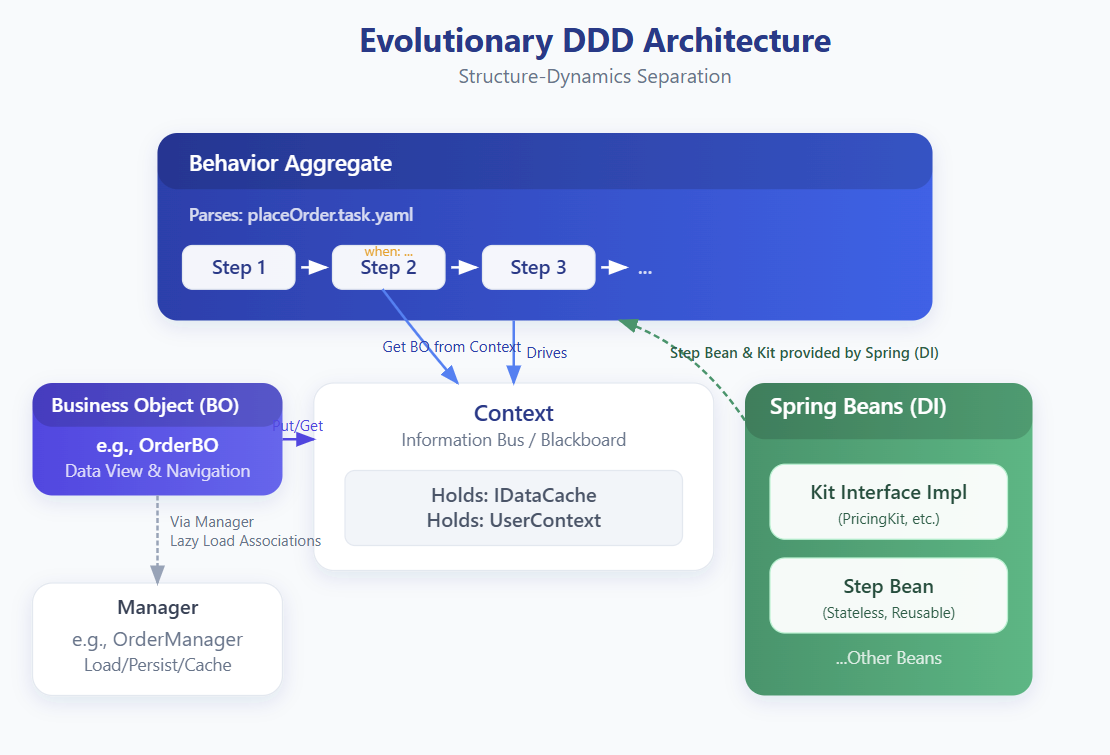
\includegraphics[width=\textwidth]{ddd/nop-ddd-arch.png}
    \caption{Evolutionary DDD Architecture after Refactoring with GRC Principles. This architecture diagram illustrates the core principle of "separating structure from dynamics." The \textbf{Behavior Aggregate} (top) is responsible for process orchestration, driven by a declarative DSL (e.g., a YAML file) and executed by a series of stateless `Step Bean`s (right). The \textbf{Data Aggregate} (the `BO` on the left) evolves into a pure, pull-based information view, with its loading and persistence managed by a `Manager`. The two are decoupled and interact via a central \textbf{Context} object (middle). The entire architecture integrates seamlessly with DI containers like Spring (right).}
    \label{fig:nop_ddd_arch}
\end{figure}

\paragraph{3. Evolution and Customization: The Application of Deltas ($\Delta$)}
When providing a customized process for a specific banking client (e.g., "Customer A"), there is \textbf{no need to modify any of the standard product's code or configuration}. One simply provides a "delta" YAML file (i.e., $\Delta$), declaratively replacing or adding steps using `x-extends`.

\begin{lstlisting}[language=YAML, caption={Customization Delta Model for Customer A}]
# === \_delta/customer-a/placeOrder.task.yaml (Customer A's Customization) ===
# Delta: Customer A's delta model, inheriting from the standard process
x:extends: /placeOrder.task.yaml
steps:
  # 1. Replace: Replace the standard credit validation with a specific version
  - x:override: replace
    name: creditValidation
    bean: customerAValidateCreditStep

  # 2. Add: After the stock check, add a fraud check step for Customer A
  - name: customerAFraudCheck
    bean: customerAFraudCheckStep
    x:insert-after: stockChecking
\end{lstlisting}
When deploying the system for "Customer A," one simply needs to set the environment's `deltaId` to `customer-a`. The Nop Platform's loader will automatically recognize the `x:extends` directive, merge the standard product's base model `/placeOrder.task.yaml` (Base) with Customer A's delta model `\_delta/customer-a/placeOrder.task.yaml` ($\Delta$) in memory, generate the final process model that meets Customer A's requirements, and then deliver it to the process engine for execution.

This case clearly demonstrates the immense engineering value of GRC principles:
\begin{itemize}
    \item \textbf{Complexity Governance}: Decomposes large, entangled business logic into clear, orthogonal units.
    \item \textbf{Evolvability}: Achieves truly non-invasive extension and customization through "delta" models, perfectly resolving the core "standardization vs. customization" conflict in software product lines.
    \item \textbf{Theory into Practice}: It translates the abstract formula $\text{App} = \text{Generator}\langle\text{DSL}\rangle \oplus \Delta$ into a concrete, actionable engineering practice that seamlessly integrates with existing tech stacks, providing a systematic solution for the efficient delivery of B2B software.
\end{itemize}

\subsection{Comparative Analysis: GRC vs. Traditional Composite Architecture}

The case study in the previous section not only demonstrates the application of GRC but also provides a concrete context for comparing the GRC paradigm with the industry's mature \textbf{Traditional Composite Architectures}. As mentioned earlier (Section 2.2.6), the latter are typically a combination of technologies like plugins, the Strategy pattern, and feature flags. Now, using the "order placement process" as an example, we will delve into the fundamental differences between the two paradigms in engineering practice.

Let's assume we are dealing with a well-designed "Before" version that already uses the Strategy pattern for credit validation and feature flags to control a new risk control feature. Even so, GRC still offers a different solution in three core dimensions.

\paragraph{1. Variability Anchors: From "Reserved Interfaces" to "Model as Coordinates"}
\begin{itemize}
    \item \textbf{Traditional Approach}: In the `OrderService`, a developer must \textbf{foresee} that credit validation is variable and thus call a strategy interface at that point. This is a \textbf{pre-defined extension point}. If a new business requirement arises, such as "add an anti-fraud scan for specific customers after the stock check," and the `placeOrder` method in `OrderService` does not have a hook pre-defined at that location, the only option is to \textbf{modify the source code of `OrderService`}.
    \item \textbf{GRC Approach}: In the GRC paradigm, the process model `placeOrder.task.yaml` is itself a \textbf{complete coordinate system}. We do not need to foresee all changes. When the anti-fraud scan needs to be added, we simply declare `x:insert-after: stockChecking` in the delta model. The target of the change (`stockChecking`) is an existing coordinate in the model, and the action of the change (`insert-after`) is an operator in the delta algebra. The entire process \textbf{requires no modification to any base Java code}.
\end{itemize}

\paragraph{2. Composition Mechanism: From "Imperative Branching" to "Declarative Merging"}
\begin{itemize}
    \item \textbf{Traditional Approach}: A user's final process flow is determined at runtime by a dynamic combination of multiple `if-else` conditions scattered throughout the code. When multiple dimensions of variability exist, these imperative branches intertwine into a complex logical web, making it difficult to fully reason about the system's behavior.
    \item \textbf{GRC Approach}: Each dimension of variability corresponds to a separate delta model ($\Delta$). The final process for a complex scenario is calculated at load-time through a deterministic algebraic operation: $\text{Base} \oplus \Delta_1 \oplus \Delta_2 \dots$. The composition logic is converged into the unified $\oplus$ merge operator, rather than being dispersed in `if` statements.
\end{itemize}

\paragraph{3. Decision Timing: From "Runtime Decisions" to "Load-time Pruning"}
GRC's management of Feature Flags is a concentrated manifestation of its difference from traditional methods.
\begin{itemize}
    \item \textbf{Traditional Approach}: Feature flags are typically checked at runtime, which means that inactive code paths still exist in the final runtime code.
    \item \textbf{GRC Approach}: GRC transforms runtime branching into \textbf{load-time model pruning}. The Nop Platform achieves this through the `feature:on` meta-attribute. For example:
    \begin{lstlisting}[language=YAML, caption={Declarative Feature Toggle in a GRC Model}]
# === placeOrder.task.yaml (Base Model) ===
# ...
steps:
  # ...
  - name: newFraudDetection
    bean: newFraudDetectionStep
    feature:on: "features.new-fraud-detection.enabled"
  # ...
    \end{lstlisting}
    The value of the `feature:on` attribute is a boolean expression. During the N (Node) phase of the S-N-V loading process, any model node that does not satisfy this condition is \textbf{completely pruned from the model tree}. This "load-time pruning" brings significant advantages: a simpler runtime with shorter execution paths and the ability to statically analyze the effective model configuration for any combination of features.
\end{itemize}

\textbf{In summary}, the case study shows that GRC offers a paradigm shift. It guides engineers from "how to deal with change by writing imperative code and pre-defining interfaces" to "how to build declarative models for the business domain and systematically compose and evolve these models through algebraic operations."

\section{Conclusion}

This paper has systematically proposed and elucidated Generalized Reversible Computation (GRC), a new paradigm aimed at unifying software construction and evolution. Unlike traditional reversible computation, which focuses on bijective logic at runtime, GRC creatively extends the principle of "reversibility" to the entire lifecycle of software construction. Its theoretical core lies in elevating the \textbf{Delta} to a computable and composable first-class citizen.

We established GRC's core construction formula, $\text{App} = \text{Generator}\langle\text{DSL}\rangle \oplus \Delta$, and argued for its recursive, fractal-like self-similarity across the vertical, horizontal, temporal, and meta-levels of software construction. By drawing an analogy with the "Dirac Picture" in physics, we have positioned GRC as a high-level computational framework for managing complexity. The main contributions of this paper are:

\begin{enumerate}
    \item \textbf{Establishing a Unified Theoretical Framework}: By introducing the concepts of a generator, an algebraic delta, and a semantic coordinate system, GRC provides a unified explanation for various technological explorations like MDE and FOP, revealing them as "unconscious" approximations toward the complete form of GRC.
    \item \textbf{Providing a Systematic Engineering Methodology}: Through the canonical implementation of the Nop Platform, we have demonstrated how to translate abstract theory into concrete engineering practice, addressing the challenges of cost, integration, and debugging when introducing a new paradigm.
    \item \textbf{Demonstrating Powerful Explanatory and Practical Value}: By reinterpreting DDD and analyzing a case study of a large-scale banking core system transformation, we have validated GRC's significant advantages in taming business complexity and achieving a harmonious coexistence of "standardization and customization."
\end{enumerate}

We believe that GRC offers a systematic, scalable, and theoretically sound solution to the two fundamental problems in software engineering: "complexity" and "evolution." It invites us to re-examine and reorganize our construction activities from a new, first-principles-based perspective, pushing software development from a "craftsmanship" model toward more predictable, industrialized production.

\section{Discussion and Future Work}

As a new paradigm, the universality of GRC theory and its engineering effectiveness have been preliminarily validated. However, every powerful theory has its application boundaries and inherent challenges. This section aims to frankly discuss the limitations of GRC, clarify some common misconceptions, and look ahead to future research directions.

\subsection{Discussion}

\subsubsection{Applicability Boundaries and the Cost of Modeling}

The core of the GRC paradigm lies in placing the construction and evolution of software systems within a structured model space defined by DSLs. Therefore, the boundary of GRC's effectiveness is essentially determined by one core question: \textbf{To what extent is an organization or project willing to "model" its business world?}

For systems that require long-term evolution and have extensive reuse and customization needs (such as software product lines), GRC provides a systematic solution. The upfront investment in modeling is compensated by high maintainability, extensibility, and automation, yielding significant long-term benefits.

However, for one-off scripts or exploratory development with highly ambiguous requirements, the structural cost of forced modeling may outweigh its benefits. It is worth noting, though, that even for seemingly unsuitable \textbf{algorithm-intensive or performance-sensitive systems}, GRC can offer value. The kernel of many high-performance systems (like databases) is itself a complex code generator, which is highly isomorphic to GRC's $\text{Generator}\langle\text{DSL}\rangle$ pattern. GRC's $\Delta$ then provides a more systematic alternative to the classic "Generation Gap Pattern" for customizing this generation logic.

\subsubsection{Complexity Management and Paradigm Fusion}

GRC is often misunderstood as adding unnecessary complexity. In reality, it does not eliminate complexity but rather \textbf{transfers, reduces, and effectively manages} it through strategies of "phase separation" and "paradigm fusion." It transfers implicit logic scattered in imperative code into declarative DSL models and reduces "glue code" through code generation.

A core advantage of GRC is its seamless fusion of declarative and imperative programming. In its core formula, the DSL does not need to be Turing-complete. When a declarative model is insufficient, the delta $\Delta$ allows for the introduction of an imperative "escape hatch," such as a script. This endows the system with the ability to handle arbitrary complexity while strictly constraining it within local, explicit delta units.

Furthermore, although GRC requires a new mental model, its engineering implementation (such as the XDef metamodel in the Nop Platform) greatly reduces the cost of this transition. Once an architect defines a business DSL using XDef, the platform **immediately and automatically** endows this new language with the full suite of GRC capabilities.

\subsection{Future Work}

Based on the discussion above, we believe that future research and development in GRC can focus on the following directions:

\begin{enumerate}
    \item \textbf{Formalization of Delta Algebra}: This paper provides a conceptual framework and engineering implementation for GRC. The next critical step is to establish a rigorous formal model for this delta algebra. This includes an axiomatic definition for its core operator $\oplus$, formal proofs of properties like associativity, and exploring the completeness of the algebraic structure.
    \item \textbf{Integration of AI and GRC}: GRC provides an ideal "scaffolding" for AI-assisted programming. $\text{Generator}\langle\text{DSL}\rangle \oplus \Delta$ offers a structurally clear and verifiable construction target. Future research can explore leveraging LLMs to automatically generate DSL models, intelligently recommend deltas, and even reverse-engineer models from legacy code.
    \item \textbf{Optimization of Toolchains and Developer Experience}: Continuously invest in developing smarter IDE plugins, visual delta comparison tools, and interactive learning tutorials to lower the learning curve of the GRC paradigm.
    \item \textbf{Broader Case Studies and Theoretical Corroboration}: Apply the GRC paradigm to a wider variety of software systems to test and expand the boundaries of its theoretical applicability and to find more evidence of "convergent evolution" in independent practices.
\end{enumerate}

We believe that by confronting its limitations and continuing to explore, Generalized Reversible Computation has the potential to grow from a novel theoretical paradigm into a mature infrastructure that profoundly changes the way software is produced. The related open-source implementation and further documentation can be found at \url{https://github.com/entropy-cloud/nop-entropy}, and we welcome community contributions and collaboration.


\begin{thebibliography}{99}

\bibitem{landauer1961}
Landauer, R. (1961). Irreversibility and heat generation in the computing process. \textit{IBM Journal of Research and Development, 5}(3), 183-191.

\bibitem{bennett1973}
Bennett, C. H. (1973). Logical reversibility of computation. \textit{IBM Journal of Research and Development, 17}(6), 525-532.

\bibitem{omg2003}
Object Management Group (OMG). (2003). \textit{MDA Guide Version 1.0.1}. OMG Document ab/2003-06-01.

\bibitem{schmidt2006}
Schmidt, D. C. (2006). Model-driven engineering. \textit{IEEE Computer, 39}(2), 25-31.

\bibitem{batory2004}
Batory, D., Sarvela, J. N., \& Rauschmayer, A. (2004). Scaling step-wise refinement. \textit{IEEE Transactions on Software Engineering, 30}(6), 355-371.

\bibitem{schaefer2010}
Schaefer, I., \& Czarnecki, K. (2010). Delta-Oriented Programming of Software Product Lines. In \textit{Software Product Lines: Going Beyond} (pp. 95-120). Springer.

\bibitem{pohl2005}
Pohl, K., Böckle, G., \& Van Der Linden, F. J. (2005). \textit{Software product line engineering: foundations, principles, and techniques}. Springer.

\bibitem{kaestner2009}
Kästner, C., Apel, S., \& Batory, D. (2009). A case study implementing a domain-specific language for feature-oriented programming. \textit{International Journal on Software Tools for Technology Transfer, 11}(5), 403-421.

\bibitem{kiczales1997}
Kiczales, G., Lamping, J., Mendhekar, A., Maeda, C., Lopes, C., Loingtier, J. M., \& Irwin, J. (1997). Aspect-oriented programming. In \textit{ECOOP'97 -- Object-Oriented Programming} (pp. 220-242). Springer.

\bibitem{gousios2013}
Gousios, G. (2013). The GHTorrent dataset and tool suite. In \textit{Proceedings of the 10th Working Conference on Mining Software Repositories} (pp. 233-236).

\bibitem{foster2007}
Foster, J. N., Greenwald, M. B., Moore, J. T., Pierce, B. C., \& Schmitt, A. (2007). Combinators for bidirectional tree transformations: A linguistic approach to the view-update problem. \textit{ACM Transactions on Programming Languages and Systems (TOPLAS), 29}(3), 17.

\bibitem{pixar2016}
Pixar Animation Studios. (2016). Universal Scene Description: A System for Composing and Collaborating on Animated 3D Scenes. \textit{ACM SIGGRAPH 2016 Talks}.

\bibitem{evans2004}
Evans, E. (2004). \textit{Domain-Driven Design: Tackling Complexity in the Heart of Software}. Addison-Wesley Professional.

\bibitem{fowler2010dsl}
Fowler, M. (2010). \textit{Domain-Specific Languages}. Addison-Wesley Professional.

\bibitem{erdweg2013}
Erdweg, S., van der Storm, T., Völter, M., Boersma, M., Bosman, R., Cook, W. R., ... \& Visser, E. (2013). The state of the art in language workbenches. In \textit{Software Language Engineering} (pp. 197-217). Springer.

\bibitem{fowler2005lw}
Fowler, M. (2005). Language workbenches: The killer-app for domain specific languages?. \textit{martinfowler.com}. Retrieved from \url{https://martinfowler.com/articles/languageWorkbench.html}

\bibitem{dmitriev2004}
Dmitriev, S. (2004, October). Language oriented programming: The next programming paradigm. In \textit{Companion to the 19th annual ACM SIGPLAN conference on Object-oriented programming, systems, languages, and applications} (pp. 122-130).

\end{thebibliography}

\appendix

\section{The Choice and Construction of Delta Space}

The core formula of GRC theory, $\text{App} = \text{Base} \oplus \Delta$, mathematically raises a fundamental question: in which "space" should we define the delta ($\Delta$) and its merge operator ($\oplus$)? This choice is crucial as it directly determines the engineering value of GRC theory.

At the most fundamental level, any software entity can be represented as a string of binary bits. In \textbf{binary space}, the equation $\text{App} = \text{Base} \oplus \Delta$ is always solvable. If we define $\oplus$ as the bitwise XOR operation, then the delta $\Delta$ can be precisely calculated:
\[
\Delta = \text{Base} \oplus \text{App}
\]
This is because the XOR operation satisfies the associative and nullifying properties: $\text{Base} \oplus (\text{Base} \oplus \text{App}) = (\text{Base} \oplus \text{Base}) \oplus \text{App} = 0 \oplus \text{App} = \text{App}$.

However, although binary space is theoretically complete, its engineering value is extremely limited. A binary delta of a function is completely unreadable and incomprehensible to a human developer.

Another common space is the \textbf{line-based text space}, which is the space where version control tools like Git operate. In this space, deltas manifest as line additions, deletions, and modifications (`diff/patch`). This type of delta is human-readable, but the line-based text space is disconnected from business semantics and is very "fragile." For example, reformatting code can produce a massive, meaningless "delta," creating significant noise.

The profound insight of GRC theory is this: \textbf{we must actively "design and construct" a delta space that has good mathematical properties and clear business semantics}. This space is the model space defined by a \textbf{Domain-Specific Language (DSL)}.

\begin{itemize}
    \item The success of \textbf{Docker} can be seen as its clever choice of the \textbf{filesystem} as its core delta space. A Docker image layer is a filesystem-level delta ($\Delta$). The vast technological assets (like OverlayFS) built around the filesystem by the Linux community naturally became the \textbf{generators} and operators in this space.
    \item The practice of \textbf{GRC (as in the Nop Platform)}, on the other hand, constructs a series of independent, semantically clear \textbf{domain model spaces} by defining a set of XDSLs (for business processes, UI pages, data models, etc.). In these spaces, deltas are structured, business-meaningful node changes, and their merge rules (`x-extends`) are designed to be algebraically complete.
\end{itemize}

Therefore, the essence of GRC is not to passively accept a given representation space, but to \textbf{actively and intentionally construct a superior delta space} that makes the process of software construction and evolution more precise, controllable, and automated.

\section{Implementation Mechanism of the Delta Merge Operator \texttt{x-extends}}

The core operator $\oplus$ of GRC theory is implemented as `x-extends` in the Nop Platform. Its powerful delta merging capability is built on a layered, coarse-to-fine implementation mechanism that covers two levels: from the filesystem to the internal structure of files.

\subsection{Two-Layer Delta Mechanism: From File Overlay to Internal Fusion}
The implementation of `x-extends` combines two delta strategies:
\begin{enumerate}
    \item \textbf{File-Level Delta (Overlay)}: A macroscopic overlay mechanism based on a \textbf{Virtual File System (VFS)}. It determines which file version to use based on the priority of different "layers."
    \item \textbf{Intra-File Delta (Merge)}: A microscopic merge mechanism. Inside structured files like XML, JSON, or YAML, it performs precise node-level additions, deletions, and modifications based on meta-directives like `x:override`.
\end{enumerate}

\subsection{File-Level Delta: Virtual File System and Delta Layers}
The Nop Platform implements a VFS that supports "delta layers." All application resources are accessed through the VFS. The path resolution in the VFS considers a global `deltaId` parameter, which specifies the currently active delta layer.

\textbf{Example Directory Structure}:
\begin{verbatim}
/_vfs/                           <-- VFS Root
  /_delta/customer-a/            <-- Delta layer for Customer A
    /beans/core.xml
  /_delta/customer-b/            <-- Delta layer for Customer B
    /config/auth.json
  /beans/core.xml                <-- Base product file
  /config/auth.json              <-- Base product file
\end{verbatim}

\textbf{Working Mechanism}:
When the system runs with `deltaId=customer-a` and requests access to `/beans/core.xml`, the VFS first checks if `/\_delta/customer-a/beans/core.xml` exists. If it does, this file is returned. If not, the VFS falls back to the base layer. This is similar to Docker's OverlayFS.

\subsection{Intra-File Delta: Structured Merge Algorithm}
When the VFS locates a delta file containing a directive like `x:extends="super"`, the intra-file merge algorithm is triggered.

\textbf{Example}:
\begin{lstlisting}[language=XML, caption={Base Definition (`/beans/core.xml`)}]
<beans>
    <bean id="securityManager" class="com.mycorp.StandardSecurityManager"/>
    <bean id="dataService" class="com.mycorp.DefaultDataService"/>
</beans>
\end{lstlisting}

\begin{lstlisting}[language=XML, caption={Customer A's Delta Definition (`/\_delta/customer-a/beans/core.xml`)}]
<beans x:extends="super">
    <!-- 1. Modify attribute -->
    <bean id="securityManager" class="com.customer.AdvancedSecurityManager"/>

    <!-- 2. Remove node -->
    <bean id="dataService" x:override="remove"/>
    
    <!-- 3. Add new node -->
    <bean id="auditLogger" class="com.customer.AuditLogger" />
</beans>
\end{lstlisting}

\textbf{Core Logic of the Merge Algorithm (Pseudocode)}:
The following is a simplified, illustrative version of the recursive Delta merge algorithm.

\begin{lstlisting}[language=PythonPseudocode, caption={Simplified Delta Merge Algorithm}]
function merge(base_node, delta_node):
    # 1. Check the override directive on the delta node
    override_action = delta_node.getAttribute('x:override')

    if override_action == 'remove':
        return NULL  # Mark for deletion
    
    if override_action == 'replace':
        return delta_node # Complete replacement

    # 2. Default action is MERGE
    result_node = base_node.clone()

    # 3. Merge attributes: Delta's attributes override Base's
    for attr_name, attr_value in delta_node.getAttributes():
        result_node.setAttribute(attr_name, attr_value)

    # 4. Merge child nodes
    base_children_map = build_map_by_key(base_node.getChildren())
    delta_children_map = build_map_by_key(delta_node.getChildren())

    new_children = []
    
    # Iterate through the order of the base model's children
    for base_child in base_node.getChildren():
        child_key = base_child.getKey()
        
        if child_key in delta_children_map:
            # Found a matching child in Delta, merge recursively
            delta_child = delta_children_map[child_key]
            merged_child = merge(base_child, delta_child)
            if merged_child is not NULL:
                new_children.append(merged_child)
            del delta_children_map[child_key]
        else:
            # No match in Delta, keep the base child
            new_children.append(base_child)
            
    # 5. Append any remaining, unmatched nodes from Delta as new additions
    for remaining_delta_child in delta_children_map.values():
        new_children.append(remaining_delta_child)
    
    result_node.setChildren(new_children)
    
    return result_node

# Helper to build a map based on a unique key (id, name, x:id)
function build_map_by_key(nodes):
    # ... implementation ...
\end{lstlisting}

\textbf{Key Points of the Algorithm}:
\begin{itemize}
    \item \textbf{Coordinate Location}: The core is to find a stable unique identifier (like `id`, `name`) for each element in a collection to establish coordinates.
    \item \textbf{Recursive Merging}: The algorithm recursively calls itself to perform a deep merge on matching nodes.
    \item \textbf{Order Preservation}: The algorithm attempts to preserve the original order of elements from the base model.
\end{itemize}

\section{An Argument for the Associativity of the Merge Operator $\oplus$}

The mathematical foundation of GRC theory is delta algebra. To make the Delta a "first-class citizen" that is independently composable and reusable, its merge operator $\oplus$ \textbf{must be designed to satisfy} associativity:
\[
(\Delta_1 \oplus \Delta_2) \oplus \Delta_3 = \Delta_1 \oplus (\Delta_2 \oplus \Delta_3)
\]
Associativity ensures that the order of delta merging is irrelevant, which allows us to process deltas in parallel and locally. This appendix provides an intuitive argument and design rationale for associativity.

\subsection{The Domain Model Coordinate System}
GRC treats any structured software artifact as a \textbf{domain model} and establishes a \textbf{domain coordinate system} for it. Every value in the model can be located by a unique \textbf{Path}. For example, for the XML:
\begin{lstlisting}[language=XML, numbers=none]
<entity name="MyEntity">
  <columns><column name="status" length="10" /></columns>
</entity>
\end{lstlisting}
We can "flatten" it into a `{path: value}` map:
\begin{verbatim}
{
  "/@name": "MyEntity",
  "/columns/column[@name='status']/@length": 10
}
\end{verbatim}
All GRC operations are essentially operations on the values at specific coordinate points.

\subsection{The Argument for Associativity}
If we view a model as a high-dimensional vector where each dimension corresponds to a unique domain coordinate, then the merge of two models $M_1 \oplus M_2$ can be seen as a dimension-wise merge of two vectors. To \textbf{argue} that the merge of vectors satisfies associativity, we only need to \textbf{show} that the value merge operation at a single coordinate point satisfies associativity.

Let $\oplus$ be the value merge operator at a single coordinate point. The most fundamental merge semantic in GRC is \textbf{Override}: $A \oplus B = B$.
Its associativity can be intuitively demonstrated:
\begin{align*}
(A \oplus B) \oplus C &= B \oplus C = C \\
A \oplus (B \oplus C) &= A \oplus C = C
\end{align*}
Therefore, $(A \oplus B) \oplus C = A \oplus (B \oplus C)$. \textbf{A merge operation based on override naturally satisfies associativity.} The GRC `x-extends` operator is designed based on conditional overrides, and thus also satisfies associativity.

\subsection{The Independence of Deltas and the Inverse Element}
A common question is: how can a delta that "deletes field C" (an inverse element $-\Delta$) exist independently of a base model that does not contain field C? The key is to distinguish between the \textbf{logical world} and the \textbf{physical world}.
\begin{enumerate}
    \item \textbf{In the logical world, deltas are complete and closed}. A delta that "deletes field C" can be logically merged with another delta that "modifies the type of field C" beforehand.
    \item \textbf{Projection from the logical to the physical world}. When we "materialize" the merged logical model, we introduce a \textbf{Projection} operator. If the final model contains an operation to "delete field C," but the base model does not have this field, the operation is \textbf{safely ignored}.
\end{enumerate}
In the Nop Platform's implementation, this is handled through meta-attributes like `x:override="remove"`. This "logically closed, physically projected" mechanism ensures that deltas are \textbf{independent and composable} in the logical world, while being \textbf{safe and robust} in the physical world.

\section{XDSL--The Engineering Carrier for the GRC Paradigm}

The construction formula of GRC, $\text{App} = \text{Generator}\langle\text{DSL}\rangle \oplus \Delta$, is realized in engineering through a set of universal language specifications called XDSL. The core design of XDSL is to embed the \textbf{Delta ($\Delta$)} and the \textbf{Generator} directly into a tree-like structure that has a stable coordinate system.

\subsection{Structured Delta ($\Delta$) and Merge Operator ($\oplus$)}
XDSL provides native delta merging capabilities for all DSLs through a set of common `x:` meta-attributes.
\begin{itemize}
    \item \textbf{`x:extends`}: Defines a file as a \textbf{Delta ($\Delta$)}.
    \item \textbf{`x:override`}: Controls the behavior of the \textbf{Merge Operator ($\oplus$)} at the node level.
        \begin{itemize}
            \item `merge` (default): Recursively merges child nodes.
            \item `replace`: Completely replaces the base node.
            \item `remove`: Deletes the base node.
        \end{itemize}
\end{itemize}
\textbf{Example}:
\begin{lstlisting}[language=XML, caption={Delta model using XDSL attributes}]
<!-- delta.xml -->
<config x:extends="base.xml">
    <!-- The `enabled` attribute is modified -->
    <feature name="A" enabled="false"/>
    <!-- The `feature[name='B']` node is removed -->
    <feature name="B" x:override="remove"/>
    <!-- A new `feature[name='C']` node is added -->
    <feature name="C" enabled="true"/>
</config>
\end{lstlisting}

\subsection{Embedded Generator}
The $\text{Generator}\langle\text{DSL}\rangle$ is implemented through embedded `x:gen-extends` directives. The content of these directives are calls to **purely functional** Xpl tag libraries, whose output is determined solely by declarative attributes.

\textbf{Working Mechanism}: During model loading, the Xpl tags are executed, and the \textbf{XNode (Abstract Syntax Tree node)} they return is treated as a dynamically generated delta ($\Delta_{\text{generated}}$), which then participates in subsequent merges.

\begin{lstlisting}[language=XML, caption={Model with an embedded generator}]
<orm x:schema="/nop/schema/orm.xdef">
    <x:gen-extends>
        <!--
          Embedded Generator: Calls the pdman:GenOrm tag,
          which reads a JSON metadata file and transforms it 
          into a series of ORM entity nodes.
        -->
        <pdman:GenOrm src="/my-app/meta/app.pdma.json"
                      xpl:lib="/nop/orm/xlib/pdman.xlib" />
    </x:gen-extends>

    <!-- Apply a delta correction to the result of the Generator -->
    <entities>
        <entity name="MyOrder">
             <components>
                 <component name="orderSummary" class="my.OrderSummaryComponent"/>
             </components>
        </entity>
    </entities>
</orm>
\end{lstlisting}

\subsection{Deterministic Construction Order}
XDSL defines a deterministic, multi-stage delta merging pipeline. All these construction operations are completed during the model loading phase and are completely transparent to the runtime, implementing the core "phase separation" idea of GRC.

\end{document}